\documentclass{article}
\usepackage{dsfont}
\usepackage{caption}
\usepackage{amsmath}
\usepackage{amsthm}
\usepackage{amssymb}
\usepackage{amsfonts}
\usepackage{tcolorbox} % for colored box around pasage
\usepackage{graphicx}
\graphicspath{{img/}}
\usepackage[ngerman]{babel}
\usepackage[margin=2.5cm,headheight=22.28003pt,top=2.5cm]{geometry}
\usepackage{mathptmx}
\usepackage{setspace}
\usepackage{lipsum} % this package is used to create dummy text.
\usepackage{enumitem}
\usepackage[utf8]{inputenc}
\usepackage[margin=2.5cm,headheight=22.28003pt,top=2.5cm]{geometry}
\usepackage{bbm}
\usepackage[margin=2.5cm,headheight=22.28003pt,top=2.5cm]{geometry}
\usepackage{xcolor}
\usepackage{tikz}
\usepackage[margin=2.5cm,headheight=22.28003pt,top=2.5cm]{geometry}
\usepackage{mathptmx}
\usepackage{setspace}
\usepackage{amsmath}
\usepackage{mathptmx}
\usepackage{graphicx} % for graphics
\usepackage{lipsum} % for sample text
\usepackage[margin=2.5cm,headheight=22.28003pt,top=2.5cm]{geometry}
\usepackage{mathptmx}
\usepackage{setspace}
\usepackage{amsmath}
\usepackage{mathptmx}
\usepackage{graphicx} % for graphics
\usepackage{lipsum} % for sample text
\usepackage{amsthm}
\usepackage[ngerman]{babel}
%\usepackage{fontspec}
\usepackage{hyperref}
\usepackage{fancyhdr}
\usepackage{titlesec}
\usepackage[T1]{fontenc}
\usepackage{lmodern}


\pagestyle{fancy}
\fancyhf{}
\lhead{\leftmark}
\rhead{\thepage}

\hypersetup{
    colorlinks=true,
    linkcolor=blue,
    urlcolor=blue,
    citecolor=blue,
    linktoc=all
}
\newtheorem{proposition}{Proposition}

\usetikzlibrary{tikzmark}

\usetikzlibrary{automata, positioning} % Hinzufügen der benötigten TikZ-Bibliotheken
\usetikzlibrary{arrows, positioning, calc}
\newtheorem{newproposition}{Proposition}[subsection] % Propositionen werden nach Subsections nummeriert


% Funktion für ein Kapitel
\newcommand{\mychapter}[1]{%
  \chapter{#1}%
  \label{sec:\theHchapter}%
}

% Funktion für eine Section
\newcommand{\mysection}[1]{%
  \section{#1}%
  \label{sec:\thesection}%
}

% Funktion für eine Subsection
\newcommand{\mysubsection}[1]{%
  \subsection{#1}%
  \label{subsec:\thesubsection}%
}

% Funktion für eine Subsubsection
\newcommand{\mysubsubsection}[1]{%
  \subsubsection{#1}%
  \label{subsubsec:\thesubsubsection}%
}

\newcommand{\coversection}[3]{
  \clearpage % Start the section on a new page
  \thispagestyle{empty} % No page number on the section page
  
  \vspace*{2cm} % Vertical spacing
  
  \begin{center}
    %\includegraphics[width=0.5\linewidth]{#1} % Adjust the width as needed
  \end{center}
  
  \vspace{2cm} % Vertical spacing
  
  \mysection{\textbf{#2}} % Section title
  
  \vspace{1cm} % Vertical spacing
  
  \begin{flushright}
    \textit{\small #3} % Quote
  \end{flushright}  
  \vfill % Fill the remaining vertical space with whitespace
  \vspace{2cm} % Vertical spacing
  \vfill % Fill the remaining vertical space with whitespace
  \clearpage % Add an empty page after the section page
}
\begin{document}

\begin{titlepage}
  
    \centering
    \vspace*{2cm}
  
    % Uni Logo
    %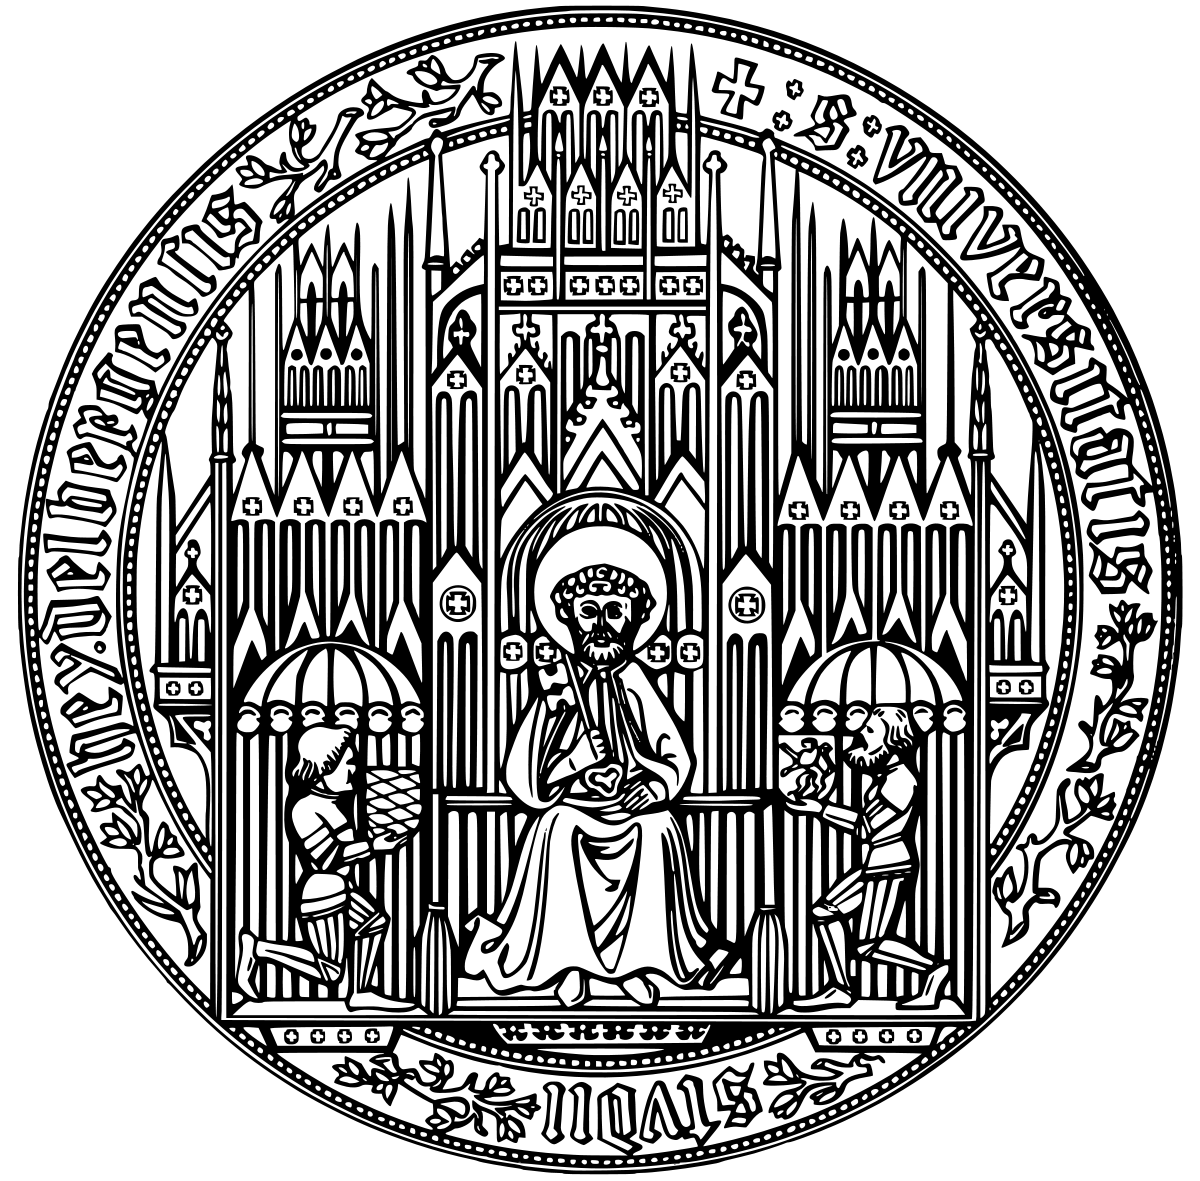
\includegraphics[width=0.3\textwidth]{unilogo.png}
    \vspace{1cm}
  
    % Course and University Information
    \textsc{\Large Einführung in die Theoretische Informatik - Script}\\[1.5cm]
    
    \title{Einführung in die Theoretische Informatik}
    \author{Lukas Dzielski\thanks{Universität Heidelberg}}
    
    \texttt{\large https://github.com/C0d3Crush/ITH-Script}\\
    \texttt{\large Lukas.Dzielski@stud.uni-heidelberg.de}\\[2cm]

    % Git Repository
    
\includegraphics[width=0.2\textwidth]{qrcode.png}\\[10cm]

  
    % Date
    {\large \today}\\[2cm]
  
    \vfill
  
\end{titlepage}

\newpage

\tableofcontents

\newpage

\begin{figure}
    \centering
    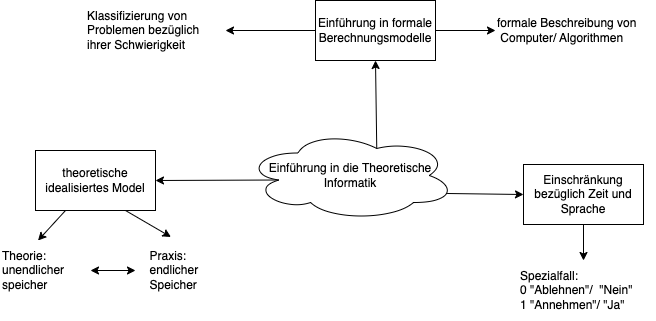
\includegraphics[width=1\textwidth]{Grundlagen/Einführung.png}
    \caption{Überblick theoretische Informatik}
    \label{fig:example}
\end{figure}

\section{Grundlagen}

\mysubsection{Notationen und begriffe}
\begin{itemize}
    \item $\mathbb{N}$ bezeichnet die \{1, 2, 3\}
    \item $\mathbb{N}_{0}$, sei $[n]$ = \{1,$\ldots $,n\} und $[n]_{0}$ = \{0, 1, $\ldots $,n\} 
    \item Für eine Menge A und n$\in \mathbb{N}$ ist $A^{n}$ = \{($a_{1},\ldots, a_{n}$): $a_{1}$, $\ldots$ $a_{n}$ $\in$ A\}
    \item Für n $\in \mathbb{N}$ ist eine n-äre partielle funktion $\varphi$ : $A^{n} \leadsto B $ eine Funktion mit dom($\varphi$) $\supseteq A^{n}$ und Im($\varphi$) $\subseteq$ B. 
    Für $a_{1}$, ..., $a_{n}$ $\in$ A bedeuted $\varphi$($a_{1}$, ..., $a_{n}$)$\downarrow$, dass ($a_{1}$, ..., $a_{n}$) $\in$ dom($\varphi$) gilt und $\varphi$($a_{1}$, ..., $a_{n}$)$\uparrow$ bedeutet, 
    dass ($a_{1}$, ..., $a_{n}$) $\notin$ dom($\varphi$). Statt $\varphi$($a_{1}$, ..., $a_{n}$)$\uparrow$ schreiben wir auch $\varphi$($a_{1}$, ..., $a_{n}$) = $\uparrow$.
    Die partielle Funktion $\varphi$ ist total, wenn dom($\varphi$) = $A^{n}$ gilt.
    \item Eine lineare Ordnung, auch totale Ordnung, auf einer Menge A ist eine Relation $\leq  \subseteq  A^{n}$m sodass die folgende Eigenschaften erfüllt sind. 
    (wie für Relationen üblich verwenden wir hier Infixntation, schreiben also für a,b $\in$ A den Ausdruck a $\leq $ b anstatt (a,b) $\in \leq $ ): 
    \begin{enumerate}
        \item[(i)] a $\leq $ a $\forall$ a $\in$ A (Reflexivität)
        \item[(ii)] a $\leq $ b $ \land $ b $\leq $ a $\Rightarrow $ a = b $\forall$a,b $\in$ A (Antisymetrie)
        \item[(iii)] a $\leq $ b, b $\leq $ c $\Rightarrow$ a $\leq $ c $forall$a,b,c $\in$ A (Transitiität)
        \item[(iv)] a $\leq $ b $\vee$ b $\leq $ a $\forall$a,b $\in$ A (Totalität)
    \end{enumerate} 
\end{itemize}

\mysubsection{Alphabet, Wörter und Sprachen}
Eingaben und Ausgaben in unseren Berechnungsmodellen werden wörter genannt, wobei wir beliebige Zeichenketten als Wörter zulassen.

\mysubsubsection{Definition (Alphabet)}
Ein Alphabet ist eine nichtleere endliche Menge $\Sigma$. Das Alphabet $\Sigma$ wird $\lvert \Sigma \rvert$- är bezeichnet. Die Elemente von $\Sigma$ heißen Buchstaben oder Symbole.

\mysubsubsection{Definition (Wörter)}
Ein Wort über einem Alphabet $\Sigma$ ist eine endliche Folge von Symbolen aus $\Sigma$. Die Länge eines Wortes w ist $\lvert$w$\rvert$. Für i $\in\lvert$w$\rvert$ bezeichnet w(i) das i-te Element von w und für Symbole $a_{1}$, $\cdots$, $a_{n} \in \Sigma$ bezeichnet $a_{1}, \cdots, a_{n}$ das Wort w der Länge n mit w(i) das i-te Element von w und für Symbole $a_{1}, \cdots, a_{n} \in \Sigma$ bezeichnet $a_{1}$, $\cdots$, $a_{n}$ das Wort w der Länge n mit w(i) = $a_{i}$ $\forall$i$\in$ \([n]\). Das Wort der Länge 0 heißt leeres Wort und wird $\lambda$ bezeichnet. Ein Wort der länge 1 wird mit dem Symbol w(1) identifiziert.

\mysubsubsection{Definition (Binäraphabet, Binärwörter)}
Das Alphabet \{0, 1\} heißt Binäralphabet. Die Wörter über dem Binäralphabet heißen Binärwörter.

\mysubsubsection{Sprache}
Eine \textbf{Sprache} ist eine Menge von Wörter über einem gemeinsahmen Alphabet $\Sigma$. Einige einfache grundlegenden Sprachen sind die folgenden.

\mysubsubsection{Definition}
Die Menge Aller Wörter über $\Sigma$ wird mit $\Sigma^{*}$ bezeichnet. Für n $\in$ $\mathbb{N}_{0}$ setzen wir:
\begin{itemize}
    \item[] $\Sigma^{\leq n}$ := \{w $\in \Sigma^{*} : \lvert$w$\rvert \leq $n\}
    \item[] $\Sigma^{=n}$ := \{w $\in \Sigma^{*} : \lvert$w$\rvert = $n\}
    \item[] $\Sigma^{\geq n}$ := \{w $\in \Sigma^{*} : \lvert$w$\rvert \geq $n\}
    \item[] $\Sigma^{+}$ := $\Sigma^{\leq 1}$
\end{itemize}

\mysubsubsection{Definition (Verkettung)}
Für Wörter $w_{1}, w_{2}$ ist die verkettung  $w_{1} \circ w_{2}$, auch $w_{1}w_{2}$, von $w_{1}$ und $w_{2}$ ist definiert durch:
\[w_{1} \circ w_{2} := w_{1} \cdots w_{1} (\lvert w_{1} \rvert)w_{2} \cdots w_{2} (\lvert w_{2} \rvert)\]
Für ein Wort w und n $\in \mathbb{N}_{0}$ ist $w^{k}$ induktiv definiert durch $w^{n}$ := $\lambda$ falls n = 0 und $w^{n}$ := $w^{n-1} \circ w^{n}$ falls n $\geq $ 1. Für eine Sprachen $L_{1}$, $L_{2}$ sei durch $L_{1} \circ L_{1}$, auch $L_{1}L_{2}$ definiert durch
\[L_{1} \circ L_{1} := \{w_{1}w_{2} : w_{1} \in L_{1}, w_{2} \in L_{2}\}\]
Für eine Sprache L und und n $\in\mathbb{N}_{0}$ ist $L^{n}$ moduliert definiert durch $L^{n} = \{\lambda\}$ falls n = 0 und $L^{n}$ := L $\cdot$ $L^{n - 1}$ falls n $\geq$ 1. Zudem sei $L^{*}$ := $\bigcup \limits_{n \in \mathbb{N}_{0}}L^{n}$. Für ein Wort w und eine Sprache L sei wL :=\{w\}$\circ$L und Lw := L$\circ$ \{w\}.\\\\Wir folgen der Konventrion, dass $\bullet^{n}$ und $\bullet^{*}$ stärker binden als 0;?? für Wörter u, v gilt also uv = u $\circ$ ($v^{n}$). Insbesondere gilt auch $ab^{n}$ = a($b^{n}$) für Symbole a, b eines Alphabets $\Sigma$.

\mysubsubsection{Definition (Präfix, Infix, Suffix)}
Seiene u, v Wörter.
\begin{itemize}
    \item [(i)] u ist Präfix von v, kurz u $\sqsubseteq $v, falls es ein Wort w gibt ,sodass $uw = v$.
    \item [(ii)] u ist Infix von v falls es Wörter $w_{1}$, $w_{1}$ gibt sodass v = $w_{1} u w_{2}$
    \item [(iii)] u ist Suffic von v, falls es ein Wort w gibt, sodass $v = wu$.
\end{itemize}

\mysubsubsection{Definition (präfixfrei)}
Eine Sprache heißt \textbf{präfixfrei}, wenn $u\sqsubseteq v \Rightarrow u = v \forall u,v \in L$.

\mysubsubsection{Definition (Homomorphismus)}
Für Sprache L und M heißt eine Funktion $\varphi : L \rightarrow M$ \textbf{Homomorphismus von Sprachen}, wenn $\varphi(uv) = \varphi (u) \varphi (v) \forall u, v \in L$ gilt.

\mysubsubsection{Definition (Längenlexikographische Ordnung)} Ist $\Sigma$ ein Alphabet und $\leq $ eine lineare Ordnung auf $\Sigma$, so ist die zu $\leq $ gehörige \textbf{längenlexikographische Ordnung} $\leq_{llex}$ auf $\Sigma^{*}$ die lineare Ordnung für die $u \leq_{llex} v $genau dann für zwei verschiedene $u, v\in \Sigma^{*}$ gilt, wenn eine der folgenden Bedingungen gilt:
\begin{itemize}
    \item $\lvert u \rvert < \lvert v \rvert$
    \item $\lvert u \rvert = \lvert v \rvert$ und ist $i \in [|u|]$ minimal mit 
    $u(i) \neq v(i)$m so gilt $u(i) \leq v(i)$.
\end{itemize}
\textbf{Bemerkung: }Oft gehen wir von einer impliziten Ordnung auf $\Sigma$ aus. Ist $\Sigma = {a_{1}, \cdots, a_{n}}$ so gilt $a_{1}\leq \cdots \leq a_{n}$

\mysubsubsection{Bemerkung} Sei $\Sigma$ ein Alphabet $\forall w \in \Sigma^{*}$ ist ${v\in \Sigma^{*} : v \leq_{llex}w}$ endlich. Dies erlaubt es uns für ein Alphabet $\Sigma$ die Wörter über $\Sigma$ in längenlexilographischen Reihenfolge $w_{1}, w_{2}, \cdots$ zu betrachten, wobei wir $w_{i}$ für $i \in \mathbb{N}$ als kleinstes Element von $\Sigma^{*}/{w_{1},\cdots, w_{i-1}}$ gewählt sei. Wir identifizieren oft $\mathbb{N}_{0}$ mit ${0, 1}^{*}$ indem wir $i \in \mathbb{N}_{0}$ mit in die längenlexilographische Reihenfolge $(i+1)$-ten Wort $w_{i+1} \in {0,1}^{*}$ identifiziernen.
\begin{center}
    \begin{tabular}{ c c c c c }
        $\mathbb{N}_{0}$ & $0$ & $1$ & $2$ & $3$\\ 
        $\{0, 1\}^{*}$ & $\lambda$ & $0$ & $1$ & $00$\\   
    \end{tabular}
\end{center}

\mysubsubsection{Definition} Es bezeichnet $bin : \mathbb{N}_{0} \rightarrow \{0, 1\}^{*}$ die Funktion, für die $bin(i)$ das in längenlexikographischer Reihenfolge (i+1)-te Binärwort ist $\forall i \in \mathbb{N}_{0}$

\mysubsubsection{Bemerkung}
$\forall i \in \mathbb{N}_{0}$ ist $1 bin(i)$ die Binärdarstellung von i+1. Umgekehrt ist $\forall w \in {0, 1}^{*}$ das $(2^{|w|} + \underset{i \in [|w|]}{\Sigma} w(i) 2^{|w|-i})$-te Binärwort.

\coversection{Turingmachine/turing.png}{Turingmachine}{A Turing machine is like a wise old person, sitting at an endless table, playing a complex game. They have a magical pen that reads and writes on the game board. They follow strict rules, do not move from their spot, but the table mysteriously moves back and forth. Their concentration is deep and calm as they perform a complex ballet of reading, writing, and state-changing.\\ \hspace*{\fill} - ChatGPT}Wir Betrachte das folgende, sehr bekannt, berechnunsmodell. Anschaulich lässt es sich wie folht beschreiben.
\begin{itemize}
  \renewcommand\labelitemi{-}
  \item Es gibt einen "Speicher" $\leadsto $ k unendlich lange Arrays(\textbf{Bänder})
  \item Es gibt einen "Arbeitsspeicher" $\leadsto$ eine endliche Menge von Zusänden, die die Machine einnehmen kann
  \item Für jedes Band gibt es einen Schreib- und Lesekopf 
  \item Jeder Schritt ist wie folgt:\\ Abhängig von Zustand und gelesenene Symbol, Schreiben die Küpfe genau ein Symbol, bewegen sich nun maximal eine Position und der Zustand der Machine wird geändert.
  \item Stellt die Machine ihhr schrittweises Arbeiten ein, so wird die Ausgabe entweder den Zustand entnommen oder von einem der Bänder in geeigneter Weise abgelesen.
\end{itemize}

\begin{figure}[htp]
  \centering
  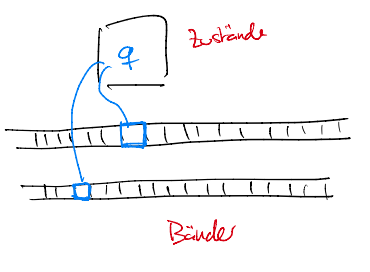
\includegraphics[width=0.5\textwidth]{Turingmachine/turing_sym.png}
  \caption{Turingmachine.}
  \label{fig:tm}
\end{figure}

\mysubsection{Definition (Turingmachine, Alan Tuing, 1936)} Sei $k \in \mathbb{N}$ eine \textbf{k-Band-Turingmachine}m kurz k-TM, ist ein Tupe $M = (Q, \Sigma, \varGamma, \Delta, s, F )$. Dabei ist:
\begin{itemize}
  \item Q eine endliche Menge, \textbf{Zustandmenge}
  \item $\Sigma$ das \textbf{Eingabealphabet}, ein Alphabet $\Box \not \in \Sigma$
  \item $\varGamma$ das \textbf{Bandaphabet}, ein Alphabet mit $\Sigma \subseteq \varGamma$ und $\Box \in \varGamma / \Sigma$ 
  \item $\Delta \subseteq Q \times \varGamma^{k} \rightarrow \subseteq Q \times \varGamma^{k} \times {L, S, R}^{k}$ die \textbf{Übergangsrelation}
  \item $s \in Q$ der \textbf{Startzustand}
  \item $F \subseteq Q$ die Menge der \textbf{akzeptierenden Zustände} 
\end{itemize}
\begin{sloppypar}
  \noindent Das Symbol $\Box$ heißt \textbf{Blank}. Die Elemente von $\Delta$ heißen \textbf{instruktionen}. Für eine Instruktion $(q_{1}, a_{1}, \cdots, a_{k}, q', a'_{1}, \cdots, a'_{k}, B_{1}, \cdots, B_{k})$ \textbf{Anweisungteil}. Die TM M ist eine \textbf{deterministische k-Band Turingmachine}, kurz k-DTM, wenn es $\forall b \in Q \times \varGamma^{k}$ höchstens eine Instruktion $i \in \Delta$ mit Bedingungsteil b.
\end{sloppypar}

\mysubsection{Definition (Konfiguration)} Sei $M = (Q, \Sigma, \Gamma, \Delta, s, F)$ eine k-TM. EIne \textbf{Konfigration} von M ist ein Tupel \[C = (q, w_{1}, \cdots, w_{k}, p_{1}, \cdots, p_{k}) \in Q \times (p^{*})^{k} \times \mathbb{N}^{k}\] Die \textbf{Startkonfiguration} von M zur Eingabe $(u_{1}, \cdots, u_{n}) \in (\Sigma^{*})^{n}$, wobei $n \in \mathbb{N}$, ist die Konfiguration \[Start_{M}(u_{1}, \cdots, u_{n}) = (s, u_{1} \Box u_{2} \Box \cdots \Box u_{n}, \Box, \cdots, 1, \cdots, 1)\] Die Konfiguration C ist eine \textbf{Stoppkonfigration} von M, wenn es keine Instruktion $i \in \Delta$ mit Bedingungsteil $(q, w_{1}(p_{1}), \cdots, w_{k}(p_{k}))$ gibt.

\mysubsection{Definition (Nachfolgekonfiguration)} 
\begin{sloppypar}
  Sei $M = (Q, \Sigma, \Gamma, \Delta, s, F)$ eine k-DTM. Für Konfiguration $C = q_{1}, w_{1}, \cdots, w_{k}, p_{1},\cdots, p_{k}$ und $C' = q'_{1}, w'_{1}, \cdots, w'_{k}, p'_{1},\cdots, p'_{k}$ von M ist die Konfigration C' Nachfolgekonfiguration von C, wenn es eine Instruktion \[(q, w_{1}(p_{1}), \cdots, w_{k}(p_{k}), a_{1}', a_{k}', B_{1}, \cdots, B_{k}) \in \Delta\] gibt, sodass 
\end{sloppypar}
\begin{equation*}
  w_{i}' = 
  \begin{cases}
    \Box a_{i}' w_{i}(2) \cdots w_{i}(|w_{i}|), & \text{falls}\ p_{i} = 1 \text{und}  B_{i} = L \\
    w_{i} \cdots w_{i}(|w_{i}| - 1) a_{i}' \Box, & \text{falls}\ p{i} = |w_{i}| \text{und} B_{i} = R \\
    w_{i} \cdots w_{i}(p_{i}-1) a_{i}' w_{i}(p_{i} + 1) \cdots w_{i}(|w_{i}|), & \text{sonst} \\
  \end{cases}
\end{equation*}
und 
\begin{equation*}
  p_{i}' = 
  \begin{cases}
    1, & \text{falls}\ p_{i} = 1 \text{ und } B_{i} = L\\
    p_{i} - 1, & \text{falls}\ p_{i} \geq 2 \text{ und } B_{i} = L\\
    p_{i}, & \text{falls}\ B_{i} = S\\
    p_{i} + 1, & \text{falls}\ B_{i} = R\\
  \end{cases}
\end{equation*}
$\forall i \in [k]$ gelten. \\ Es bezeichnen $\rightarrow M$ die Relation auf der Menge der Konfiguration von M, sodass $C \rightarrow_{M} C'$ falls C, C' Konfig von M sind wobei C' eine Nachfolgekonfiguration von C ist.

\mysubsection{Definition (Rechnung)} Sei $M = (Q, \Sigma, \Gamma, \Delta, s, F)$ eine k-DTM. Eine \textbf{endliche partielle Rechnung} von M ist eine endliche Folge $C_{1}, \cdots, C_{n}$ von Konfig von M mit $C_{i} \rightarrow_{M} C_{i+1} \forall i \in [n-1]$. Eine \textbf{unendliche partielle Rechnung} von M ist eine unendliche Folge $C_{1}, C_{2}, \cdots$ von Konfigration von M mit $C_{1} \rightarrow_{M} C_{1+1} \forall i \in \mathbb{N}$. Eine \textbf{Rechnung von M zur Eingabe } ($w_{1}, \cdots
, w_{n}) \in (\Sigma^*)^n$ (mit $n \in \mathbb{N}$) ist eine endliche partielle Rechnung $start_M = C_1, \cdots, C_m$ bei der $C_m$ eine Stoppkonfiguration von M oder eine unendliche partielle rechnung $start_M(w_1, \cdots, w_n) = C_1, C_2, \cdots$

\mysubsection{Bemerkung} Ist M eine k-DTM, so gilt es $\forall n \in \mathbb{N}$ und $(w_1, \cdots, w_n) \in (\Sigma^*)^n$ genau eine Rechnung zur Eingabe $(w_1, \cdots, w_n)$.

\mysubsection{Definition (total)} Eine k-DTM $M = (Q, \Sigma, \Gamma, \Delta, s, F)$ \textbf{terminiert} bei Eingabe $(w_1, \cdots, w_n) \in (\Sigma^*)^n$ wenn die Rechnung von M zur Eingabe $(w_1, \cdots, w_n)$ endlich ist. Eine k-TM $M = (Q, \Sigma, \Gamma, \Delta, s, F)$ ist \textbf{total}, wenn $\forall n \in \mathbb{N}$ und $(w_1, \cdots, w_n) \in (\Sigma^*)^n$ alle Rechnungen von M zur Eingabe $(w_1, \cdots, w_n)$ endlich sind.

\mysubsection{Definition (akzeptierte Sprache)} Sei $M = (Q, \Sigma, \Gamma, \Delta, s, F)$ eine k-TM. Eine Stoppkonfiguration $(q, w_1, \cdots, w_k, p_1, \cdots, p_k)$ von M ist \textbf{akzeptierend}, wenn $q \in F$. Die \textbf{akzeptierte Sprache L(M)} von M ist die Sprache über dem Alphabet $\Sigma$ so dass $w\in L(M)$ gilt, wenn es eien endliche Rechnung $C_1, \cdots, C_n$ von M zur Eingabe w gibt, bei der $C_n$ eine akzeptierende Stoppkonfigration von M ist. \\ \textbf{Hinweis: } Für nicht deterministische TM heißt das insbesondere, dass es für die Wörter w in der akzeptierten Sprache nur mindestend \textbf{eine} im einer akzeptierten Stoppkonfigration endende endliche Rechnung zur Eingabe w geben muss. Für Wörter w, die nicht in L(M) sind, sind \textbf{alle} rechnungen von M zur Eingabe am Ende nicht in einer akzeptierten Stoppkonfigration oder unendlich.

\mysubsection{Definition(entscheidbar)}
Eine Sprache L ist genau dann \textbf{entscheidbar}, wenn es eien totale k-TM M mit L(M) = L gibt. Wir schreiben \textbf{REC} für die Klasse der entscheidbaren Sprachen. Der Begriff entscheidbar für Sprachen ergibt sich hier daraus, dass effektiv entschieden werden kann ob eine gegebene Eingabe in der Sprache liegt oder nicht. Insbesondere steht? dies voraus, dass Eingabe, die nicht in der Sprache liegen effektiv als nicht in der Sprache liegend erkannt werden. \\ \textbf{Begriff: } effektiv $\leadsto$ eine TM erlefigt dies in endicher Zeit. Da sich der durch TM formatierte Berechenbarkeitsbegriff, also die Formalisierung dessen was effektiv durchführbar ist, auch äquivalent durch rekursive Funktion definieren lässt, weden entscheidbare Sprachen auch als rekuriv bezeichnet.

\mysubsection{Definition(rekursiv aufzählbar)} Eine Sprache L ist genau dann \textbf{rekursiv aufzähbar}, wenn es eine k-TM mit akzeptierten Sprache L gibt. Wir schreiben \textbf{RE} für die Klasse der rekursiv aufzählbaren Sprachen. Die Aufzählbarkeit leitet sich daraus ab, dass es für eine rekuriv aufzählbare Sprache L über einem Alühabet $\Sigma$ möglich ist effektive Verfahren anzugeben ,die die Wörter von L aufzählen, also dass eine endlich oder unendliche Aufzählung von $A = w_1, w_2, \cdots$ mit ${w_1, w_2, \cdots} = L$ existiert.\\\\
\textit{"Rekursiv aufzählbar" ist ein Begriff der verwendet wird um eine Menge zu beschreiben, die wir mit einem Computerprogramm oder Algorithmus "auflisten" können.
Stellen Sie sich vor, Sie haben eine Box mit nummerierten Bällen, und Sie haben ein Programm, das Bälle aus der Box zieht. Wenn Sie sicherstellen können, dass Sie jeden Ball in der Box mindestens einmal ziehen, egal wie lange es dauert, dann ist die Menge der Bälle in der Box "rekursiv aufzählbar }\\\\
\textit{Wenn wir sagen, dass eine Sprache "rekursiv aufzählbar" ist, bedeutet das, dass es einen Algorithmus oder ein Computerprogramm gibt, das alle Wörter in dieser Sprache "auflisten" kann. Es könnte einige Wörter mehrmals auflisten und es könnte eine sehr lange Zeit dauern, aber es würde schließlich jedes Wort in der Sprache "treffen".
Eine "k-TM" ist eine Art von Maschine, die wir in der theoretischen Informatik verwenden, um diese Art von Aufzählung zu machen. Wenn es eine k-TM gibt, die eine Sprache akzeptiert, bedeutet das, dass die Sprache rekursiv aufzählbar ist.}
\mysubsection{Bemerkung} Jede entscheidbare Sprache ist rekursiv aufzähbar.

\mysubsection{Bemerkung} Alle endlichen Sprachen sind entscheidbar.

\mysubsection{Bemerkung} Eine Sprache L über einem Alphabet $\Sigma$ist genau dann entscheidbar, wenn $L$ und $L^c :=(\Sigma^*)/L$ rekursiv aufzähbar sind.

\mysubsection{Definition (Ausgabe)} Sei $M = (Q, \Sigma, \Gamma, \Delta, s, F)$ eine k-TM und $C = (q, w_1, \cdots, w_k, p_1, \cdots, p_k)$ eine Konfigration von M. Die Ausgabe $out_M(C)$ von M bei Konfiguration C ist das Präfix $w \sqsubseteq w_1(p_1), \cdots, w_1(|w_1|)$ maximale Länge mit $w \in (\Gamma / {\Box})^*$.

\mysubsection{Definition (berechnete Funktion)} Sei $M = (Q, \Sigma, \Gamma, \Delta, s, F)$ eine k-DTM und $n \in \mathbb{N}$. Die von M berechnete \textbf{n-äre partielle Funktion} $\Phi_M$ ist die partielle Funktion $\Phi_M : (\Sigma^*)^n \leadsto (\Gamma / {\Box})^*$, so dass $\forall (w_1, \cdots, w_n) \in (\Sigma^*)^n$ folgendes gilt:
\begin{enumerate}
  \item Ist die rechnung von M zur Eingabe $(w_1, \cdots, w_n)$ die endliche Rechnung $C_1, \cdots, C_M$, so gilt $\Phi_M(w_1, \cdots, w_n) = out_M(C_M)$.
  \item Ist die Rechnung von M zur Eingabe $(w_1, \cdots, w_n)$ unendlich, so gilt $\Phi_M(w_1, \cdots, w_n)\uparrow $
\end{enumerate}
Für $w_1, \cdots, w_n \in \Sigma^*$ schreiben wir statt $\Phi_M(w_1, \cdots, w_n)$ auch $M(w_1, \cdots, w_n)$.

\mysubsection{Definition (partiell berechenbar)}
Für Alphabet $\Sigma, \Gamma$ und eine partielle Funktion $\Phi : \Sigma^* \leadsto \Gamma^*$ ist $\Phi$ \textbf{partiell berechenbar}, wenn es eine $k \in \mathbb{N}$ gibt und eine k-DTM M mit $\Phi_M = \Phi$ gibt. Ist $\Phi $total und partiell berechenbar, so ist $\Phi$ berechenbar. Wir schreiben \textbf{RF} für die Klasse der partiellen Funktionen.\\\\Mittels der Induktivität von $\mathbb{N}_0$ und ${0, 1}^*$ können so auch partielle Funktionen, die von oder nach $\mathbb{N}_0$ abbilden als (partielle) berechenbare Funktion bezeichnent werden. Beispielsweise ist eine partielle Funktion $\Phi : \mathbb{N}_0 \leadsto \mathbb{N}_0$ dennoch genau dann partiell berechenbar, wenn die partielle Funktion $bin \circ \Phi \circ bin^-1$ partiell berechenbar ist. Gewissermaßen verfügen die hier definierten TM über zewi Ausgabemechanismen. Die Ausgabeim engeren Sinne in Definition 2.13 und das Ablesen vn Akzeptanz anhand des schließlich erreichten Zustands in Definition 2.7. Im Sinne der folgenden Bemerkung wäre der zweiten Fall nicht notwendig, allerdings ist dies ein wichtiger spezialfall.

\mysubsection{Definition (charackteristische Funktion, partielle charachteristische Funktion)} Sei L eine Sprache über dem Alphabet $\Sigma$
\begin{itemize}
  \item [(i)] Die \textbf{charackteristische Funktion} von L als Sprache über $\Sigma$ ist die Funktion $\mathbbm{1}_L : \Sigma \rightarrow \{0, 1\}$ mit $\mathbbm{1}_L = 1$ $\forall w \in L$ und $\mathbbm{1}_L (u) = 0$ $\forall w \in \Sigma^* / L$.
  \item [(ii)] Die \textbf{ partielle charackteristische Funktion} von L als Sprache über $\Sigma$ ist die partielle Funktion $x_L : \Sigma^* \leadsto \{1\}$ mit $x_L(w) = 1$ $\forall w \in L$ und $x_L(w) \uparrow$  $\forall w \in \Sigma^* / L.$ 
\end{itemize}

\mysubsection{Bemerkung} Sei L eine Sprache über einem Alphabet $\Sigma$. 
\begin{itemize}
  \item [(i)] L ist genau dann entscheidbar, wenn $\mathbbm{1}_L$ berechenbar ist.
  \item [(ii)] L ist genau dann rekursiv aufzähbar, wenn $x_L$ partiell berechenbar ist.
\end{itemize}

\mysubsection{Bemerkung (normiert)} Eine 1-DTM $M = (Q, \Sigma, \Gamma, \Delta, s, F)$ heißt \textbf{normiert}, wenn $Q = {0,\cdots, n}$ für eine $n \in \mathbb{N}_{0}$, $\Sigma = {0, 1}$, $\Gamma = {\Box, 0, 1}$, $s = 0$, $F = {s}$. Alle TMs mit Eingabealphabet ${0,1}$ lassen sich mit folgenden Schritten in eine normierte TM mit gleicher erkannter Sprache und gleicher berechneter Funktion umwandeln. 
\begin{itemize}
  \item Von Nichtdeterminismus zu Determinismus: Eine DTM kann die Rechnungen einer nichtdeterministischen TM parallel im Sinne von abwechend schrittweise durchführen um schließlich das Verhalten der simulierten TM zu ??. Dies entspricht einer \textbf{Breitensuche im Rechnungsbaum}. 
  \begin{center}
    \begin{tikzpicture}[
      level distance=1.5cm,
      level 1/.style={sibling distance=3cm},
      level 2/.style={sibling distance=1.5cm},
      every node/.style={align=center}]
      
      \node (0) {$wort_M(w)$}
        child {node (1) {$C_1$}
          child {node (3) {$C_3$}}
          child {node (4) {$C_4$}}
        }
        child {node (2) {$C_2$}
          child {node (5) {$C_5$}}
          child {node (6) {$C_6$}}
        };
    
      \path[->,red,thick] (0) edge (1)
                           (1) edge (2)
                           (2) edge (3)
                           (3) edge (4)
                           (4) edge (5)
                           (5) edge (6);
    \end{tikzpicture}
\end{center}
  \item Von mehreren Bändern zu einem Band: Intuitiv können k Bänder auf ein Band simuliert werden, indem die Felder des einen Bandes in k-teilfelder unterteilt werden, die jeweils die gleiche Bandalphabetbuchstaben wie zufor als Beschreibung zulassen und es zudem erlaubt zu markieren, dass der simulierte Kopf des simulierten Bandes dort steht. Eine dieser Idee folgende Konstruktion wird als \textbf{Spurentechnik} bezeichnet. Formal: Übergang vom Bandalphabet $\Gamma$ zu \[((\Gamma \cup{\underline{a} : a \in \Gamma})^{k}/{\Box}^{k}) \cup {\Box}\] 
  wobei $\underline{a} \not \in \Gamma$ für $a \in \Gamma$. Hierbei bedeutet \underline{a}, dass das simulierte Feld mit a beschriftet ist und dass dort der simulierte Kopf steht. Weiter spielt $\Box$ die Rolle des k-Tupels $(\Box, \cdots, \Box)$ um der Tatsache gerecht zu werden, dan alle Felderzu Begin mit $\Box$ beschriftet sind.
  \begin{center}
    \begin{tikzpicture}[cell/.style={rectangle, draw=black, minimum size=1cm}, node distance=0cm]

      % Erstes Band
      \node[cell] (cell11) {...};
      \node[cell, right=of cell11, draw=red] (cell12) {0};
      \node[cell, right=of cell12] (cell13) {0};
      \node[cell, right=of cell13] (cell14) {1};
      \node[cell, right=of cell14] (cell15) {...};
      
      % Zweites Band
      \node[cell, below=0.5cm of cell11] (cell21) {...};
      \node[cell, right=of cell21] (cell22) {1};
      \node[cell, right=of cell22] (cell23) {0};
      \node[cell, right=of cell23, draw=red] (cell24) {0};
      \node[cell, right=of cell24] (cell25) {...};
      
      % Drittes Band
      \node[cell, below=0.5cm of cell21] (cell31) {...};
      \node[cell, right=of cell31] (cell32) {0};
      \node[cell, right=of cell32, draw=red] (cell33) {1};
      \node[cell, right=of cell33] (cell34) {1};
      \node[cell, right=of cell34] (cell35) {...};
      
      % Vertikales Band
      \node[cell, right=5cm of cell22, minimum height=4.13cm, align=center] (cell41) {...};
      \node[cell, right=0cm of cell41, minimum height=4.13cm, align=center, draw=red] (cell42) {1 \\\\\\ 0 \\\\\\ 1};
      \node[cell, right=0cm of cell42, minimum height=4.13cm, align=center] (cell43) {1 \\\\\\ 0 \\\\\\ 1};
      \node[cell, right=0cm of cell43, minimum height=4.13cm, align=center] (cell44) {1 \\\\\\ 0 \\\\\\ 1};
      \node[cell, right=0cm of cell44, minimum height=4.13cm, align=center] (cell45) {...};


      % Pfeil
      \draw[->, very thick] ([yshift=0.25cm]cell12.north) -- (cell12.north);

      % Pfeil
      \draw[->, very thick] ([yshift=0.25cm]cell24.north) -- (cell24.north);

      % Pfeil
      \draw[->, very thick] ([yshift=0.25cm]cell33.north) -- (cell33.north);

      % Pfeil
      \draw[->, very thick] ([yshift=0.25cm]cell42.north) -- (cell42.north);

      % Buchstabe am Pfeil
      \node[above=0.2cm of cell12.north] {$\varphi$};

      % Buchstabe am Pfeil
      \node[above=0.2cm of cell42.north] {q};

      % Pfeil von links nach rechts über den Bändern
      \draw[->, very thick, black] (cell25.east) -- (cell41.west);

      \end{tikzpicture}
      
  \end{center}
    
  \item Von beliebigen bandalphabet zu $\{\Box, 0, 1\}$: Andere bandalphabete können bei einem \textbf{Alphabetwechel} zum Bandalphabet $\{\Box, 0, 1\}$ simuliert werden um ein Symbol des vorherigen Bandlaphabets durch ein Binärwort zu beschreiben. Die TM liest stets nur ein Feld, es wird dabei also nötig sein die Zustandsmenge so zu erweitern, dass angrenzende Felder im Zustand gespeichert weden können.
  
  \usetikzlibrary{arrows, positioning, calc}
\begin{center}
  \begin{tikzpicture}[cell/.style={rectangle, draw=black, minimum size=1cm}, arrow/.style={->, >=stealth, thick, shorten <=1pt, shorten >=1pt}, dashedline/.style={dashed, shorten <=1pt, shorten >=1pt}]

    % Oberes Band
    \foreach \i/\label in {1/A,2/B,3/C,4/D,5/E,6/F,7/G} {
      \node[cell] (ucell\i) at (\i, 0) {\label};
    }
    
    % Unteres Band
\foreach \i/\label in {0/1,1/2,2/3,3/4,4/5,5/6,6/7,7/8,8/9,9/10,10/11,11/12,12/13,13/14} {
  \node[cell] (lcell\i) at (\i/2+0.25, -3.5) {\label};
}
    
    % Verbindungslinien
    \foreach \i in {1,...,7} {
        \pgfmathtruncatemacro\j{2*\i-2}
        \pgfmathtruncatemacro\k{2*\i-1}
        \draw[dashedline] (ucell\i.south west) -- (lcell\k.north west);
    }
    
    % Pfeil auf die erste Zelle
    \draw[arrow] (1,2) -- (ucell1);

    \end{tikzpicture}
\end{center}

\end{itemize}

\mysubsection{Bemerkung} Sei $L \subseteq \{0, 1\}^*$ eine Sprache und sei $\Phi : \{0, 1\}^* \leadsto \{0, 1\}^*$ eine partielle Funktion.
\begin{itemize}
  \item [(i)] L ist genau dann entscheidbar, wenn L akzeptierte Sprache einer totalen normierten TM ist. 
  \item [(ii)] L ist genau dann rekursiv aufzähbar, wenn L akzeptierte Sprache einer normierten TM ist.
  \item [(iii)] $\Phi$ ist genau dann partiell berechenbar, wenn $\Phi$ berechnete Funktion einer normierten TM ist.
\end{itemize}

\mysubsection{Church- Turing- These} Berechenbarkeit auf eienr Turingmachine entspricht intuitiver Berechenbarkeit.

\coversection{Berechenbarkeit/predic.png}{Berechenbarkeit}{Predictability is like knowing the path a river takes. The river starts at its source and flows down to the sea. Along the way, it may turn, twist, and divide, but it always follows the path of least resistance due to gravity. Knowing the terrain allows us to predict where the river will go.\\ \hspace*{\fill} - ChatGPT}
\textbf{Konvention: } Sprechen wir von einer $e \in \mathbb{N}_0$ oder $(e_1, \cdots, e_n) \in \mathbb{N}_0^n$ wobei $n \in \mathbb{N}$ als Eingabe für eine TM oder Ausgabe einer TM, so bedetet dies, dass die Eingabe bzw. Ausgabe $bin(e)$ bzw $(bin(e_1), \cdots, bin(e_n))$ ist. Dies erlaubt es über partiell berechnenbare Funktionene $\Phi: \mathbb{N}_0^n \leadsto \mathbb{N}_0$ wobei $n\in \mathbb{N}$ zu sprechen und $L \subseteq \mathbb{N}_0$ als Sprache über $\{0, 1\}$ aufzufassen.

\mysubsection{Definition (Code)} Wir betrachten die Funktion code (mit geeignetem Definitionsbereich) und Zielmenge $\{0, 1\}^*$, für die folgendes gilt. Zunächst gelte \[code(L) = 10 \qquad code (S) = 00 \qquad code(R) = 01\] Für eine Instruktion $ I = (q, a, q', a', B) \in \mathbb{N}_0 \times \{0, 1\} \to \mathbb{N}_0 \times \{0, 1\} \times \{L, S, R\}$ einer normierten TM sei \[code (I) = 0^{|bin(q)|} 1 bin (q) a 0^{|bin(q')|} 1 bin (q') a' code (B)\] Für eine endliche Menge $ \Delta \subseteq \mathbb{N}_0 \times \{0, 1\} \to \mathbb{N}_0 \times \{0, 1\}\times \{L, S, R\}$ von Instruktionen einer normierten TM und $i \in [|\Delta|]$ sein $code_i(\Delta)$ dann ein längenlexikographische Ordnung i-te Wort in $\{code(I): I \in \Delta\}$ und sei \[ code (\Delta) = code_1(\Delta), \cdots, code_{|\Delta|}(\Delta)\] Für eine normierte TM $M = (\{0, \cdots, n\}, \{0, 1\}, \{\Box, 0, 1\}, \Delta, 0, \{0\})$ sei \[ code (M) = 0^{|bin(n)|} 1 bin (n) code (\Delta)\] der \textbf{Code} von $M$. Relevant ist hierbei dass es eine geeignete effektive Codierung von Turingmachinen durch Binärwörter gibt, so dass folgendes gilt 
\begin{itemize}
  \item Jede normierte TM hat einen Code 
  \item Keine zwei verschiedene normierten TMs haben den gleichen Code.
  \item Die Sprache der Codes von Turingmachinen ist entscheidbar
  \item Codes können eine geeignete Repräsentation der durch sie codierten TMs umgewandelt werden, die es insbesondere erlauben die codierten TMs effekiv zu simulieren.
  \item geignete Repräsentationen von TMs können effektiv in ihre Codes umgewandet werden.
\end{itemize}

\mysubsection{Definition (standardaufzählung)} Sei $\hat{w_0}, \hat{w_1}, \cdots$ die Aufzählung aller Codes normierter TMs in längenlexikographischer Ordnung. Für $e \in \mathbb{N}_0$ sei $M_e$ die durch $\hat{w_e}$ codierte TM und für $n \in \mathbb{N}$ sei $\Phi_e^n : \mathbb{N}_0^n \rightarrow \mathbb{N}_0$ die von $M_e$ berechnete n-äre partielle Funktion. Für $n \in \mathbb{N}$ heißt die Folge $(\Phi_e^n)$ mit $e\in \mathbb{N}$ \textbf{standardaufzählung} der n-ären partiell berechenbaren Funktion. Für $n \in \mathbb{N} $ und eine partiell berechenbare n-äre Funktion $\varphi: \mathbb{N}_0^n \rightarrow \mathbb{N}_0$ heißt jede zahl $e \in \mathbb{N}_0$ mit $\Phi_e^n = \varphi$ \textbf{Index} von $\varphi$.

\textbf{Konvention: } Ergibt sich n aus dem Kontext, so schreiben wir auch $\Phi_e$ statt $\Phi_e^n$

\mysubsection{Bemerkung} Für $n \in \mathbb{N}$ und eine partielle berechnbare n-äre partielle Funktion $\Phi : \mathbb{N}_0^n \rightarrow \mathbb{N}_0$ gibt es unendlich viele Indizes von $\varphi$.

\mysubsection{Definition (U)} Es bezeichnet U die normierte TM, die bei Eingabe $(e, x_1, \cdots, x_n) \in \mathbb{N}_0^{n+1}$ wobei $n \in \mathbb{N}$ die normierte TM $\mathcal{M}_e$ bei Eingabe $(x_1, \cdots, x_n)$ simuliert und falls diese terminiert die Ausgabe der Simulierten ausgibt.

\mysubsection{Definition (Universell)} Eine DTM U heißt \textbf{Universell}, wenn es für alle $n \in \mathbb{N}$ und alle partiell berechenbaren Funktionen $\varphi : \mathbb{N}_0^n \leadsto \mathbb{N}_0$ eine $e \in \mathbb{N}$, so dass \[U(e, x_1, \cdots, x_n) = \varphi(x_1, \cdots, x_n)\] $\forall x_1, \cdots, x_n \in \mathbb{N}_0$ gilt.

\mysubsection{Bemerkung} \sloppy Die TM U ist universell, denn für $e \in \mathbb{N}_0$, $n \in \mathbb{N}$ und $x_1, \cdots, x_n \in \mathbb{N}_0$ gilt \[U(e,x_1, \cdots, x_n) = \Phi_e(x_1, \cdots, x_n)\]\\ \[(x, y) \mapsto x^y\] \[y \mapsto 2^y\] \[(x_1, \cdots, x_m, y_1, \cdots, y_n) \mapsto \varphi(x_1, \cdots, x_m, y_1, \cdots, y_n) partiell berechenbar\] \[\leadsto (y_1,\cdots, y_m) \mapsto \varphi(x_1, \cdots, x_m, y_1, \cdots, y_n) partiell berechenbar \]

\mysubsection{Satz ($s_n^m$ - Theorem)} 
$\forall m, n \in \mathbb{N}$ existiert eine berechenbare Funktion $s_n^m : \mathbb{N}_0^{m+1} \to \mathbb{N}_0$  mit \[\Phi_e^{m+1}(x_1\cdots, x_m, y_1, \cdots, y_n) = \Phi_{s_n^m(e, x_1, \cdots, x_m)}^n (y_1, \cdots, y_n)\] $\forall e, x_1, \cdots, x_m, y_1, \cdots, y_n \in \mathbb{N}_0$

\begin{proof}Fixiere $m \in \mathbb{N}$. Betrachte die DTM S , die bei Eingabe $(e, x_1, \cdots, x_m) \in \mathbb{N}_0^{m+1}$ wie folgt vorfährt.
\begin{itemize}
  \item Zunächst bestimmt S den Code von $\mathcal{M}_e$ 
  \item der Code von $\mathcal{M_e}$wird dann in einen Code einer normierten TM $\mathcal{M}$ umgewandet, die zunächst $x_1\Box\cdots\Box x_m\Box$ neben die Eingabe schreibt, dan den Kopf auf das erste Feld des beschriebenen Bandteilsbewegt und dann wie $\mathcal{M_e}$ arbeitet.
  \item Es wird bestimmt an welcher Stelle der Standardaufzählung der Code von auftaucht und diese Stelle wird ausgegeben.
\end{itemize}
Sei $s_n^m$ die von S berechnete $(m+1)$-äre partielle Funktion. Dann ist $s_n^m$ eine Funktion wie gewünscht. Es gibt überabzählbar viele Binärsprachen, denn: Betrachte Aufzählung von Binärsprachen $L_1, L_2, \cdots$ 
\begin{table}[ht]
  \centering
  \renewcommand{\arraystretch}{2} % Adjust the value to increase or decrease the cell size
  \begin{tabular}{c c c c c}
    \tikzmarknode{L0-0}{$\mathds{1}_{L_0}(0)$} & $\mathds{1}_{L_0}(1)$ & $\mathds{1}_{L_0}(2)$ & $\mathds{1}_{L_0}(3)$ \\
    $\mathds{1}_{L_1}(0)$ & $\mathds{1}_{L_1}(1)$ & $\mathds{1}_{L_1}(2)$ & $\mathds{1}_{L_1}(3)$ \\
    $\mathds{1}_{L_2}(0)$ & $\mathds{1}_{L_2}(1)$ & \tikzmarknode{L2-2}{$\mathds{1}_{L_2}(2)$} & $\mathds{1}_{L_2}(3)$ \\
  \end{tabular}
  \captionsetup{labelformat=empty, justification=centering, skip=10pt}
  \caption{Standardaufzählung}
  
  \begin{tikzpicture}[overlay, remember picture, red, >=stealth]
    \draw [->, thick] ([yshift=1ex]L0-0.south) -- ([yshift=-1ex]L2-2.north);
  \end{tikzpicture}
\end{table}

$L$ mit $\mathds{1}_L(i)$ = 
$\begin{cases}
    0, & \text{wenn } \mathds{1}_{L_i}(i) = 1 \\
    1, & \text{wenn } \mathds{1}_{L_i}(i) = 0 \\
\end{cases}$
\end{proof}

\mysubsection{Definition (diagonales Halteproblem)} Die Menge $H_{diag} := \{e \in \mathbb{N}_0 : \Phi_e (e) \downarrow\}$ heißt \textbf{diagonales Halteproblem}.

\mysubsection{Proposition} Das diagonale Halteproblem ist rekursiv aufzählbar.
\begin{proof}
  Die DTM, die bei Eingabe $e \in \mathbb{N}_0$ wie $U$ bei Eingabe $(e, e)$ arbeitet, aber bei terminieren $1$ statt der Ausgabe von $U$ ausgibt berechnet die partielle charachteristische Funktion von $H_{diag}$. Die partielle Funktion $x_{H_{diag}}$ ist also partiell berechenbar. Die partielle Funktion $x_{H_{diag}^c}$ ist nicht partiell berechenbar, dann: Betrachte Standardaufzählung
\end {proof}
  
\begin{table}[ht]
  \centering
  \renewcommand{\arraystretch}{2} % Adjust the value to increase or decrease the cell size
  \begin{tabular}{c c c c c}
    \tikzmarknode{L0-0}{$\Phi_{L_0}(0)$} & $\Phi_{L_0}(1)$ & $\Phi_{L_0}(2)$ & $\Phi_{L_0}(3)$ \\
    $\Phi_{L_1}(0)$ & $\Phi_{L_1}(1)$ & $\Phi_{L_1}(2)$ & $\Phi_{L_1}(3)$ \\
    $\Phi_{L_2}(0)$ & $\Phi_{L_2}(1)$ & \tikzmarknode{L2-2}{$\Phi_{L_2}(2)$} & $\Phi_{L_2}(3)$ \\
  \end{tabular}
  \captionsetup{labelformat=empty, justification=centering, skip=10pt}
  \caption{Standardaufzählung}
\end{table}

\begin{tikzpicture}[overlay, remember picture, green, >=stealth]
  \draw [->, thick] ([yshift=1ex]L0-0.south) -- ([yshift=-1ex]L2-2.north);
\end{tikzpicture}

$\varphi$ mit $\varphi(i)$ = 
$\begin{cases}
    \uparrow, & \text{wenn } \Phi_i(i) \downarrow\\
    \downarrow, & \text{wenn } \Phi_i(i) \uparrow \\
\end{cases}$
Wird nicht aufgezählt.

\mysubsection{Satz} Das diagonale Halteproblem ist nicht entscheidbar. 
\begin{proof}
  Angenommen $H_{diag}$ wäre entscheidbar. Dann wäre die partielle charakteristische Funktion $\varphi$ von $H_{diag}^c = \mathbb{N}_0 / H_{diag}$ partiell berechenbar, es gäbe also ein Index $e \in \mathbb{N}_0$ von $\varphi$. Es folge \[e \in H_{diag}^c \Leftrightarrow \varphi(e) \downarrow \Leftrightarrow \Phi_e(e) \downarrow \Leftrightarrow e \in H_{diag} \Leftrightarrow e \not \in H_{diag}^c\] Die ist ein Wiederspruch.
\end{proof}

\mysubsection{m-Reduktion} Für eine Sprache $A$ über einem Alphabet $\Sigma$ und eine Sprache $B$ über einem Alphabet $\Gamma$ ist A genau dann \textbf{many-one-reduzierbar}, auch \textbf{m-reduzierbar}, auf $B$, kurz $A \leq_m B$, wenn es eine berechebare Funktion. $f: \Sigma^* \to \Gamma^*$ gibt so dass \[w \in A \Leftrightarrow f(w)\in B\] $\forall w \in \Sigma^*$ gilt. Gelten $A \leq_m B$ und $B \leq_{m} A$, so sind $A$ und $B$ \textbf{many-one-äquivalent} auch \textbf{m-äquivalent}, kurz $A =_m B$.

\mysubsection{Bemerkung} 
\begin{itemize}
  \item [(i)] $\leq_m$ ist transitiv.
  \item [(ii)] Gilt $A \leq_m B$ für Sprachen $A$ und $B$ und ist $B$ entscheidbar, so ist auch $A$ entscheidbar.
  \item [(iii)] Alle entscheidbaren Sprachen L mit $\varnothing \not = L \not = \mathbb{N}_0$ und m-äquivalent.
\end{itemize}

\mysubsection{Satz} Das \textbf{initiale Halteproblem} $H_{init} = {e \in \mathbb{N}_0 = \Phi_e(0) \downarrow}$ ist nicht entscheidbar.

\subsubsection*{Idee: } suche $f:\mathbb{N}_0 \to \mathbb{N}_0$ mit $\Phi_e(e)\downarrow \Leftrightarrow \Phi_{f(e)}(0)\downarrow$ Wähle $f$ so dass $\Phi_{f(e)}(x) = \Phi_e(e)$ $\forall x \in \mathbb{N}_0$

\begin{proof}
  Sei $\psi : \mathbb{N}_0^2 \leadsto \mathbb{N}_0$ mit $\psi (e, x) = \Phi_e(e) \forall e, x \in \mathbb{N}_0$. Dann ist $\psi$ partiell berechenbar. Sei $e_0$ ein Index von $\psi$ und $s:\mathbb{N}_0^2 \to \mathbb{N}_0$ gilt. Sei $f: \mathbb{N}_0 \to \mathbb{N}_0$ mit $f(e) = s(e_0, e) \forall e /in \mathbb{N}_0$. Dann ist f berechenbar. $\forall e \in \mathbb{N}_0$ gilt. \[e \in H_{diag} \Leftrightarrow \Phi_e(e) \downarrow \Leftrightarrow \psi(e, 0) \downarrow \Leftrightarrow \Phi_{e_0}(e, 0) \downarrow \Leftrightarrow \Phi_s (e_0, e)(0)\downarrow \Leftrightarrow \Phi_{f(e)} (0)\downarrow \Leftrightarrow f(e) \in H_{init}\] Es gilt also $H_{diag} \leq_{m} H_{init}$, da $H_{diag}$ nicht entscheidbar ist, ist damit $H_{init}$ nicht entscheidbar.
\end{proof}

\textbf{Dominosteinspiel!}
\subsubsection*{Gegeben: } Endlich viele typen von Spielsteinen mit jeweils zwei beschrifteten Feldern: "oberes Feld, unteres Feld". Beschritungen sind nichtleere Wörter über einem Alphabet. Spielsteine sind vom gleichen Typ, wenn die beiden oberen Felder gleich beschriftet sind und die beiden unteren Felder gleich beschriftet sind. Es gibt von jedem Typ beliebig viele steine. 

\subsubsection*{Gesucht: }Können ein oder mehrere (aber endlich viele) Spielsteine so nebeneinander gelegt werden, dass sich oben und unten von links nach rechts gelesen das gleiche Wort ergibt?
\begin{center}
  \begin{tikzpicture}
    % Define styles for Dominoes
    \tikzstyle{domino}=[rectangle, draw, minimum width=1cm, minimum height=2cm, inner sep=0pt]
  
    % Domino (0111, 0)
    \node[domino] (d1) at (0,0) {};
    \node at ([yshift=4mm]d1.center) {0111};
    \node at ([yshift=-4mm]d1.center) {0};
  
    % Domino (1, 01)
    \node[domino] (d2) at (1.5,0) {};
    \node at ([yshift=4mm]d2.center) {1};
    \node at ([yshift=-4mm]d2.center) {01};
  
    % Domino (0, 1)
    \node[domino] (d3) at (3,0) {};
    \node at ([yshift=4mm]d3.center) {0};
    \node at ([yshift=-4mm]d3.center) {1};
  
    % Domino (0, 000)
    \node[domino] (d4) at (4.5,0) {};
    \node at ([yshift=4mm]d4.center) {0};
    \node at ([yshift=-4mm]d4.center) {000};
  
    % Domino (1, 011)
    \node[domino] (d5) at (6,0) {};
    \node at ([yshift=4mm]d5.center) {1};
    \node at ([yshift=-4mm]d5.center) {011};
  
    \end{tikzpicture}
    \vspace{1cm}\\
    \begin{tikzpicture}

      % Define styles for Dominoes
      \tikzstyle{domino}=[rectangle, draw, minimum width=1cm, minimum height=2cm, inner sep=0pt]
      
      % Domino (0111, 0)
      \node[domino] (d1) at (0,0) {};
      \node at ([yshift=4mm]d1.center) {0111};
      \node at ([yshift=-4mm]d1.center) {0};
      
      % Domino (0, 1)
      \node[domino] (d2) at (1,0) {};
      \node at ([yshift=4mm]d2.center) {0};
      \node at ([yshift=-4mm]d2.center) {1};
      
      % Domino (0, 1)
      \node[domino] (d3) at (2,0) {};
      \node at ([yshift=4mm]d3.center) {0};
      \node at ([yshift=-4mm]d3.center) {1};
      
      % Domino (0, 1)
      \node[domino] (d4) at (3,0) {};
      \node at ([yshift=4mm]d4.center) {0};
      \node at ([yshift=-4mm]d4.center) {1};
      
      % Domino (0, 000)
      \node[domino] (d5) at (4,0) {};
      \node at ([yshift=4mm]d5.center) {0};
      \node at ([yshift=-4mm]d5.center) {000};
      
      % Domino (1, 01)
      \node[domino] (d6) at (5,0) {};
      \node at ([yshift=4mm]d6.center) {1};
      \node at ([yshift=-4mm]d6.center) {01};
      
      % Arrow pointing to the leftmost domino
      \draw[->, thick] (-1.5,0) -- (d1.west);

      \end{tikzpicture}
        
  \end{center}

  \mysubsection{Definition (Postsches Korrespondenzproblem, Emil Port, 1946)} Für ein Alphabet $\Sigma$ sei eine Instanz des Postschen Korrespondenzproblems über $\Sigma$ eine endliche Teilmenge $I \subseteq (\Sigma^+)^2$. Eine Lösung für eine solche Instanz ist eine endliche Folge $(u_1, v_1), \cdots, (u_n, v_n)$ von Paaren in $I$ mit $n \geq 1$,so dass \[u_1 \cdots u_n = v_1 \cdots v_n\] Gibt es eine Lösung für eine instanz des Postschen Korrespondenzproblems, so heißt diese Instanz lösbar. Das \textbf{Postsche Korrespondenzproblem} über einem Alphabet $\Sigma$, kurz $PCP_{\Sigma}$ ist die Menge aller lösbaren Instanzen des Postschen Korrespondenzproblems über $\Sigma$.\\\\ Für ein Alphabet $\Sigma$ sei eine Instanz des modifizierten Postschen Korrespondenzproblems über $\Sigma$ ein Paar $(p, I)$, wobei $I\subseteq (\Sigma^+)^2$ eine endliche Teilmenge und $p\in I$ ein Paar von Wörtern ist. Eine Lösung für eine solche Instanz ist eine endlcihe Folge $(u_1, v_1), \cdots, (u_n, v_n)$ von Paaren ist $I$, so dass \[p = (u_1, v_1) und u_1\cdots u_n = v_1\cdots v_n\] Gibt es eine Lösung für eine Instanz des modifizierten Postschen Korrespondenzproblems so heißt diese Instanz lösbar. Das \textbf{modifizierte Postsche Korrespondenzproblem} über einem Alphabet $\Sigma$, kurz $MPCP_{\Sigma}$ ist die Menge aller lösbaren Instanzen des modifizierten Postschen Korrespondenzproblems über $\Sigma$.
  \subsubsection*{Plan: } Für Alphabet mit $|\Sigma| \geq 2$: \[H_{init} \stackrel{(3)}{\leq_m} MPCP_{\Gamma} \stackrel{(2)}{\leq_m} PCP_{\Gamma} \stackrel{(1)}{\leq_m} PCP_{\Sigma}\]
  \mysubsection{Lemma} Für ein Alphabet $\Sigma$ und $\Gamma$ mit $|\Sigma| \geq w$ gilt $PCP_{\Gamma} \leq_m PCP_{\Sigma}$
  \begin{proof}
    Wir suchen eine effektive Transformation, die jede Instanz $I$ des Postschen Korrespondenzproblems über $\Gamma$ in eine Instanz $I'$ des postschen Korrespondenzproblems über $\Sigma$ transformiert, so dass $I$ genau dann lösbar ist, wenn $I'$ lösbar ist. Seien $a_1, a_2 \in \Sigma$ verschieden und sein $b_1, \cdots, b_{|\Gamma|}$ die Elemente von $\Gamma$. Es bezeichne $\varphi : \Gamma^* \to \Gamma^*$ den eindeutigen Homomorphismus von Sprachen mit $\varphi (b_i) = a^i_1 a_2$ $\forall i \in [|\Gamma|]$. Gegeben eine solche Instanz $I$ wie oben sei $I' := \{(\varphi(u), \varphi(v)) : (u, v) \in I\}$. Die Funktion, die geeignete Codes von Instanzen $I$ auf geeignete Codes von Instanzen $I'$ abbildet ist berechenbar. Ist $(u_1, v_1), \cdots, (u_n, v_n)$ eine lösung $I$, so gilt \[\varphi(u_1) \cdots \varphi(v_1) = \varphi(u_1, \cdots, \varphi(v_n)) = \varphi(v_1, \cdots, v_n) = \varphi(v_1) \cdots \varphi(v_n)\] und somit ist $(\varphi(u_1), \varphi(v_1), \cdots, (\varphi(u_n)), \varphi(v_n))$ eine Lösung von $I'$. Die Instanz $I'$ ist also lösbar wenn $I$ lösbar ist. Ist $(u'_1, v'_1), \cdots, (u'_n, v'_n)$ eine Lösung von $I'$, so gibt es eine Folge $(u_1, v_1)\cdots (u_n, v_n)$ von Paaren in $I$ mit $\varphi(u'_i)$ und $\varphi(v_i) = v'_i$ $\forall i \in [n]$, also mit \[\varphi(u_1, \cdots, u_n) = u'_1, \cdots, u'_n = u'_1, \cdots, u'_n =\varphi(u_1, \cdots, u_n)\] Da $\varphi \vert_{\Sigma}$ injektiv und $\varphi (\Sigma)$ präfixfrei ist, ist $\varphi$ injektiv (siehe Übung), folglich gilt $u_1, \cdots, u_n = v_1, \cdots, v_n$ und somit ist $(u_1, v_1), \cdots, (u_n, v_n)$ eine Lösung von $I$. Die Instanz $I$ ist also lösbar wenn $I'$ Lösbar ist.
  \end{proof}


  \mysubsection{Lemma} Für Jedes alphabet $\Sigma$ mit $|\Sigma| \leq w$ gitl $MPCP_{\Sigma} \leq_m PCP_{\Sigma}$.
  \begin{proof}
    Sei $\Sigma$ ein Alphabet mit $|\Sigma| \geq 2$. Nach \hyperref[subsec:3.14]{Lemma 3.14}  genügt es ein Alphabet $\Gamma$ zu finden, so das $MPCP_{\Sigma} \leq_m PCP_{\Gamma}$ gilt. \\Wir suchen eine effektive Transformation , die jede instanz $(p, I)$ des modifizierten Postschen Korrespondenzproblems über $\Sigma$ in eine Instanz $I'$ des Postschen Korrespondenzproblems über einem geeignetem Alphabet$\Gamma$ transformiert, so dass $(p, I)$ genau dann lösbar ist, wenn $I'$ lösbar ist.
  \end{proof}
  \subsubsection*{Idee: }
  \begin{center}
    \begin{tikzpicture}
      \draw[blue] (0,0) rectangle (1,1) node[midway] {0};
      \draw[blue] (1,0) rectangle (2,1) node[midway] {1};
      \draw[blue] (2,0) rectangle (3,1) node[midway] {0};
      \draw[green] (3,0) rectangle (4,1) node[midway] {0};
      \draw[yellow] (4,0) rectangle (5,1) node[midway] {1};
      \draw[yellow] (5,0) rectangle (6,1) node[midway] {0};
      \draw[yellow] (6,0) rectangle (7,1) node[midway] {1};
      \draw[yellow] (7,0) rectangle (8,1) node[midway] {1};
      \draw[purple] (8,0) rectangle (9,1) node[midway] {1};
      \draw[purple] (9,0) rectangle (10,1) node[midway] {0};
      \draw[purple] (10,0) rectangle (11,1) node[midway] {1};
  
      \draw[blue] (0,1) rectangle (1,2) node[midway] {0};
      \draw[green] (1,1) rectangle (2,2) node[midway] {1};
      \draw[green] (2,1) rectangle (3,2) node[midway] {0};
      \draw[green] (3,1) rectangle (4,2) node[midway] {0};
      \draw[green] (4,1) rectangle (5,2) node[midway] {1};
      \draw[yellow] (5,1) rectangle (6,2) node[midway] {0};
      \draw[yellow] (6,1) rectangle (7,2) node[midway] {1};
      \draw[purple] (7,1) rectangle (8,2) node[midway] {1};
      \draw[purple] (8,1) rectangle (9,2) node[midway] {1};
      \draw[purple] (9,1) rectangle (10,2) node[midway] {0};
      \draw[purple] (10,1) rectangle (11,2) node[midway] {1};
    \end{tikzpicture}
  \end{center}
  ...
  Betrachte die Homomorphismus von Sprachen $\delta_{\rightarrow}$, $\delta_{\leftarrow} : \Sigma^* \rightarrow (\Sigma \cup {*})^*$ mit $\delta_{a} = a*$ und $\delta_{\leftarrow}(a) = *a$ $\forall a \in \Sigma$. Für jede Instanz $(p, I) = ((u_1, v_1), I)$ wie oben sei \[I' = \{(\delta_{\leftarrow}(u_1), *\delta_{\rightarrow}(v_1))\} \cup \{\delta_{leftarrow}(u), \delta_{rightarrow}(v):  (u, v) \in I\} \cup \{\delta_{\leftarrow}(u)*, \delta_{\rightarrow}(v): (u, v) \in I\}\] Die Funktion die geeignete Codes von Instanzen $(p, I)$ auf geeignete Codes der zugehörigen Instanzen $I'$ abbildet ist berechenbar. Gibt es eine Lösung $(u_1, v_1), \cdots, (u_n, u_n)$ von $(p,I)$ dann ist \[\delta_{\leftarrow}(u_1)\cdots \delta_{\leftarrow}(u_n)* = \delta_{\leftarrow} (u_1 \cdots u_n)*\]
  \[= \delta_{\leftarrow}(v_1 \cdots v_n)*\] \[= *\delta_{\rightarrow}(v_1 \cdots v_n)\] \[=*\delta_{\rightarrow}(v_1) \cdots \delta_{\rightarrow}(v_n)\] und folglich ist \[(\delta_{\leftarrow}(u_1), *\delta_{\rightarrow}(v_1)), (\delta_{\leftarrow}(u_2), \delta_{\rightarrow}(v_2)), \cdots, (\delta_{\leftarrow}(u_{n-1}), \delta_{\rightarrow}(v_{n-1})), (\delta_{\leftarrow}(u_{n}), \delta_{\rightarrow}(v_{n}))\] eine Lösung von $I'$. Es bleibt zu zeigen das $(p, I)$ lösbar ist, wenn $I'$ lösbar ist. Sei $\tau : (\Sigma \cup \{*\})^* \rightarrow \Sigma^*$ der Homomorphismus von Sprachen mit $\tau \vert_{\Sigma} = id_{\Sigma}$ und $\tau(*) = \lambda$. Für $(u', v') \in I'$ gilt $(\tau (u'), \tau(v')) \in I$. Sei $(u'_1, v'_1), \cdots, (u'_n, v'_n)$ eine Lösung von $I'$ und $(u'_i, v'_i) = (\tau(u'_i), \tau(v'_i))$ für $i \in [n]$. Es gilt \[\tau(u'_1) \cdots \tau(u'_n) = \tau(u'_1 \cdots u'_n) = \tau(v'_1 \cdots v'_n) = \tau(v'_1) \cdots \tau(v'_n)\] und somit ist $(u_1, v_1), \cdots, (u_n, u_v)$ eine Lösung von $I$ als Instanz des Postschen Korrespondenzproblems über $\Sigma$. Es genügt aber zu zeigen, dass $(u_1, v_1) = p $ gilt. Sei $p' = (\delta_{\leftarrow} (u_1), \not \tau (?wirklich nicht tau?) \delta_{\rightarrow}(v_1))$. Für $(u', v') \in I' / \{p'\}$ gilt $u'(1) \not = v'(1)$, da $(u'_1, v'_1), \cdots, (u'_n, v'_n)$ eine Lösung von $I'$ ist gilt also $(u'_1, v'_1) = p'$ und damit $(u_1, v_1) = (\tau(u'_1), \tau(v'_1)) = p$.

  \mysubsection{Lemma}
  Für jedes Alphabet $\Sigma$ mit $|\Sigma| \geq 2$ gilt $H_{init} \leq_m MPCP_{\Box, 0, 1, *, 6, +}$

  \begin{proof}
    Wir suchen eine effektive Transformation, die jede natürliche Zahl $e$ auf eine Instanz $(p_e,I_e)$ des modifizierten Portschen Korrespondenzproblems über $\{\Box, 0, 1, *, , +\}$ abbildet, so dass $\mathcal{M} _e(\lambda)\downarrow$ genau dann gilt, wenn $(p_e, I_e)$ lösbar ist. Sei $e \in \mathbb{N}_0$. Sei $Q$ Die Zustandsmenge und $\Delta$ die Übergangsrelation von $\mathcal{M}_e$. Es gelte also $\mathcal{M}_e = (Q, \Sigma, \Gamma, \Delta, s, F)$ für $\Sigma = \{0, 1\}$, $\Gamma = \{\Box, 0, 1\}$, $S = 0$, $F = \{0\}$ \\ Für eine Instanz $(p, I)$ des modifizierten Postschen Korrespondenzproblems über einem Alphabet bezeichnen wir eine Folge $p =  (u_1, v_1), \cdots, (u_n, v_n)$ für die $u_1 \cdots u_n \sqsubseteq v_1 \cdots v_n$ oder $v_1 \cdots v_n \sqsubset u_1 \cdots u_n$ gilt als \textbf{partielle Lösung} von $(p, I)$. Wir wollen $(p_e, I_e)$ so wählen, dass partielle Lösungen von $(p_e, I_e)$ partielle Rechungen von $\mathcal{M}_e$ entsprechen. Dabei codieren wie eine Konfiguration $(p, w, p) \in Q \times(\Gamma^*)*\mathbb{N}_0$ von $\mathcal{M}_e$ durch das Wort \[code (q, w, p) := \# w(1)\cdots w(p-q) * bin(q)* w(p) \cdots w(|w|)\#\] Im wesentlichen wollen wir erreichen, dass es genau dann für ein Wort w eine partielle lösung  $(u_1, v_1), \cdots, (u_n, v_n)$ von $(p_e, I_e)$ mit $w = v_1 \cdots v_n$ gibt, wenn $w$ Präfix der Konkation $code (C_1) \cdots code (C_n)$ der Code der Konfiguration einer partiellen Rechnung $C_1, \cdots, C_n$ von $\mathcal{M}_e$ bei Eingabe $\lambda$ ist. Eine solche partielle Lösung soll genau dann zu einer Lösung von $(p_e, I_e)$ vervollständigt werden können, wenn die durch $w$ beschriebene partielle Rechung mit einer Stoppkonfiguraion endet, alsp eine Rechung ist. Dann ist $(p_e, I_e)$ genau dann lösbar, wenn die Rechung von $\mathcal{M}_e$ zur Eingabe $\lambda$ endlich ist. \\\\ Für $q \in Q$ sei $\hat{q} : * bin(q)$\\ Als Startpaar sehen wir \[p_e = (0, 0 \# * \ *\Box\#)\] (die 0en sind nur dafür da da, damit "im?" komplment nicht leer ist.) Wir beschreiben nun die Konstruktion von $I_e$. Für jede Instruktion $(q, a, q', a', L) \in \Delta$ fügen wir folgende Paare ein \[(\# \hat{q}a, \# \hat{q}'\Box a'), (\Box \hat{q} a, \hat{q}'\Box a'), (0\hat{q}a, \hat{q}'0a')(1\hat{q}a, \hat{q}'1a')\] ein. Weiter, um unveränderte Infixe kopieren zu können fügen wir die Paare \[(\#, \#), (0, 0), (1,1), (\Box, \Box)\] ein. Nun brauchen wir noch Paare, die bei Terminierung der TM zu einer validen Instanz der $MPCP$ - Instanz führen.\\ $\leadsto \forall q \in Q \forall a \in \{\Box, 0, 1\}$ für die es keine Instruktion $(q, a, q', a', B)$ fürgen wir das Paar $(\hat{q}a, \dagger a)$ hinzu und auch \[(\dagger \Box, \dagger), (\dagger 0, \dagger), (\dagger 1, \dagger)\] \[(\Box \dagger, \dagger),(0 \dagger, \dagger),(1\dagger, \dagger)\] \[(\# \dagger \# 0, 0)\] Dies beschreibt die Konstruktion von $(p_e, I_e)$. Wir verzichten auf die einfache aber aufwändige Verfifikation, dass $\mathcal{M}_e$ genau dann bei Eingabe $\lambda$ terminiert, wenn $(p_e, I_e)$ lösbar ist.
  \end{proof}
  \mysubsection{Beispiel} Sei $e \in \mathbb{N}_0$ mit $\mathcal{M}_e = (\{0, 1\}, \{0, 1\}, \{\Box, 0, 1\}, \Delta, 0, \{0\})$, wobei $\Delta = \{(0, \Box, 1, 1, R), (1, \Box, 1, 1, L)\}$. Mitder Notation aus dem Beweis aus \hyperref[subsec:3.16]{Lemma 3.17} gilt dann [hier bild einfügen!]

  \mysubsection{Satz} Für jedes Alphabet $\Sigma$ mit $|\Sigma| \geq 2$ ist $PCP_{\Sigma}$ nicht entscheidbar. 
  \begin{proof}
    Mit \hyperref[subsec:3.16]{Lemma 3.16}, \hyperref[subsec:3.17]{Lemma 3.17} und \hyperref[subsec:3.18]{Lemma 3.18} folgt \[H_{init} \leq_m MPCP_{\Box, 0, 1, *, \#, \dagger} \leq_m PCP_{\Box, 0, 1, *, \#, \dagger} \leq_m PCP_{\Sigma}\] und damit $H_{init} \leq_m PCP_{\Sigma}$. Folglich ist $PCP_{\Sigma}$ nicht entscheidbar, da $H_{init}$ nicht entscheidbar ist.
  \end{proof}

  %alda
  \mysubsection{Fixpunktsatz, Rekusionstheorem und Satz von Rice} 
  
  Wir beschäftigen uns nun mit weiteren Konsequenzen der Standardaufzählung von TM. \[ \Phi_0, \Phi_1, \Phi_2, \cdots \] Standardaufzählung \[\Phi_{\Phi_e(0)}, \Phi_{\Phi_e(1)}, \Phi_{\Phi_e(2)}, \cdots\] andere Aufzählung $\Rightarrow$ \[\Phi_{f(0)}, \Phi_{f(1)}, \Phi_{f(2)}\]

  \mysubsubsection{Definition (Fixpunktsatz)} Ein \textbf{Fixpunkt} eine berechenbaren Funktion $f: \mathbb{N}_0 \to \mathbb{N}_0$ ist ein $e \in \mathbb{N}_0$ mit $\Phi_{f(e)} = \Phi_e$.

  \mysubsubsection{Satz (Fixpunktsatz, Hartley Rogers jr., 1967)} Alle berechenbaren Funktionen $f : \mathbb{N}_0 \to \mathbb{N}_0$ haben einen Fixpunkt.
  \begin{proof}
    $\forall e, x \in \mathbb{N}_0$ mit $\Phi_e(x) \uparrow$ sei $\Phi_{\Phi_e(x)} : \mathbb{N}_0 \leadsto \mathbb{N}_0$ die aprtiell berechenabre partielle Funktion mit $dom(\Phi_{\Phi_e(x)}) = \varnothing$. Sei $e_{\psi}$ ein Index von $\psi$. Gemäß $S_n^m$-Theorem (\hyperref[subsec:3.16]{Satz 3.7}) existiert eine berechenbare Funktion $s_1^1 : \mathbb{N}_0^2 \to \mathbb{N}_0$ mit $\Phi_{s_1^1(e_{\psi}, e)}(x) = \psi(e, x)$. $\forall e, x \in \mathbb{N}_0$.Sei $\eta : \mathbb{N}_0 \to \mathbb{N}_0$ die berechenbare Funktion mit $\eta (e) := s_1^1(e_{\psi}, e)$. Dann gilt \[\psi_{\eta(e)}(x) = \psi_{s_1^1(e_{\psi}, e)}(x) = \psi(e, x) = \Phi_{\Phi_e(e)}(x) \forall x \in \mathbb{N}_0\] also gilt \[\Phi_{\eta(e)} = \Phi_{\Phi_e (e)} (*)\] Sei $e_{f \circ h}$ ein Index der berechneten Funktion $f \circ h$ und $e_{fix} := \eta(e_{f\circ h})$. \[ \Phi_{f(e_{fix})} = \Phi_{f(\eta(e_{f \circ h}))} = \Phi_{\Phi{e_{f\circ h}} (e_{f\circ h})} \overset{(*)}{=} \Phi_{\eta(e_{f \circ h})} = \Phi_{e_\eta}\] Folglich ist $e_{fix}$ ein Fixpunkt von $f$. 
  \end{proof}
  Solche Fixpnkte wie oben sind "semandische" Fixpunkte und kein "syntaktischen" Fixpunkte. Aus dem Fixpunktsatz kann man leicht das Rekursionstheorem folgen, dsa es anschaulich erlaubt während der Konstruktion einer partiell berechebaren Funktion anzunehmen den Index der fertig definierten Funktion zu kennen. Auf Programmebene bedeutet das, das es möglich ist ein Programm so zu schreiben ,dass der fertige Quellcode im Programm zur Verfügung stelt (ohne diesen irgendwo, zum Beispiel vom Speicher des Quellcodes, einzulesen)

  \mysubsubsection{Satz (Rekursionstheorem, Stephen Cole Kleen, 1938)} 
  Für alle partielle Funktionen $\varphi : \mathbb{N}_0^2 \leadsto \mathbb{N}_0$ gibt es ein $e \in \mathbb{N}_0$ mit $\Phi_e(x) = \varphi(e, x) \quad \forall x \in \mathbb{N}_0$ 

  \begin{proof}
    Sei $e_{\varphi}$ ein index von $\varphi$. Gemäß $s_n^m$ - Theorem gibt es eine berechenbare Funktion $s_1^1 : \mathbb{N}_0^2 \to \mathbb{N}_0$ mit $\Phi_{s^1_1 (e_{\varphi}, e)} (x) = \varphi (e, x) \quad \forall x \in \mathbb{N}_0$
  \end{proof}

  Für Programme bedeutet dies die Existenz von sogenannten \textbf{Quines}. Dies sind Programme, die ihren eigenen Quellcode ausgeben (ohne diesen vom speicher zu lesen). Unsere Resultate zeigen, dass für hinreichend komplexe Programmiersprachen immer Quines existieren. Eine weitere Konsequent aus dem Fixpunktsatz ist die Einsicht, dass jede nicht triviale Programmiereigenschaft unentscheidbar ist.

  \mysubsubsection{Korollar}
  Es gibt ein $e \in \mathbb{N}_0$ mit $\Phi_e(x) = e \quad \forall x \in \mathbb{N}_0$.
  \begin{proof}
    Sei $\psi : \mathbb{N}_0^2 \leadsto \mathbb{N}_0$ die partiell berechebare Funktion mit $\psi(e, x) = e \quad \forall e, x \in \mathbb{N}_0$. Gemäß \hyperref[subsubsec:3.20.2]{Satz 3.20.2} gibt es nun ein $e \in \mathbb{N}_0$ mit $\Phi_e (x) = \psi (e,x) = e \quad \forall x \in \mathbb{N}_0$
  \end{proof}

  \mysubsubsection{Definition (Indexmenge)} 
  Eine Teilmenge $I \subseteq \mathbb{N}_0$ heißt Indexmenge, wenn $e \in I \Leftrightarrow e' \in I \quad \forall e, e' \in \mathbb{N}_0$ mit $\Phi_e = \Phi_e'$ gilt.

  \mysubsubsection{Satz (Satz von Rice, Henry Horden Rice, 1951)}
  Ist $I$ ein Indexmenge $\varnothing \not = I \not = \mathbb{N}_0$, so ist $I$ nicht entscheidbar.
  \begin{proof}
    Sei $e_0 \not \in I, e_1 \in I$ und sei $f: \mathbb{N}_0 \to \mathbb{N}_0$ die Funktion mit $f(e) = e_0 \quad \forall e \in I$ und $f(e) = e_1 \quad \forall e \in \mathbb{N}_0 / I$. (Ist $I$ entscheidbar dann ist $f$ offensichtlich berechenbar.) $\forall e \in \mathbb{N}_0$ gilt $f(e) \in I \Leftrightarrow e \not \in I$ und da $I$ eine Indexmenge ist ist somit $\Phi_{f(e)} \not = \Phi_e$. Die Funktion $f$ hat also keinen Fixpunkt. Wäre $I$ entscheidbar, so hätte $f$ aber einen Fixpunkt nach dem \hyperref[subsubsec:3.20.1]{Fixpunktsatz}.
  \end{proof}
\coversection{Automaten/finit1.png}{Automaten und Grammatiken}{Imagine you're in a city with a limited number of locations (like a park, library, cafe, etc.). You can move from one place to another following specific paths (like roads). The paths you take depend on some rules, like the time of the day, or the type of ticket you have. The places you can reach with these rules represent different states in a finite automaton, and the rules themselves act like the transition function.\\ \hspace*{\fill} - ChatGPT}

Wir wollen Turingmahinen un stark einschränken. 
wir betrahten ein Modell, das im wesentlichen ohne speicher
zurechtkommt (=Tm ohne band $\longrightarrow$  brauchen es nur für die Eingabe).
Der Ausgabemechanismus kennt nur Akzeptanz und Nichtakzeptanz.\\\\
Als TM kann der wie folgt realisiert werden:
\begin{itemize}
    \item Es ist nur ein Band erlaubt.
    \item Bei jedem Rechenschritt bewegt sich der Kopf nach rechts. Ob und wie die Felder des Bandes dabei überschreiben werden spielt dann keine Rolle, denn der Kopf kann nie zurück bewegt werden; wir lehen aber fest, dass Symbole nicht überschrieben werden. Die Symbole die des Bandalphabet $\Gamma $ neben denen des Eingabealphabets $\Sigma $ und des $\square $  Symbols ?? hat ?? spielen keine Rolle. Wir legen hier $\varGamma $ = $\Sigma \cup $ \{$\square $\} fest.
    \item Beim Einlesen des ersten $\square $ Symbols muss die Rechnung der Machine enden. Wir soll die Rechnung nicht vor dem Einlesen des ersten $\square $ Symbols enden. 
\end{itemize}
??Die?? bedeutet, dass wir DM M = (Q, $\Sigma$m $\Sigma\cup $\{$\square $\}), $\delta$, s, F) die nur Instruktionen der Form (q, a, q', a, R) mit q $\in$ Q und a $\in \sigma$ hat.
Dies sind nun stark eingeschränkte TM. Wir wählen eine äquivalente Form, die als endliche Automaten bezeichnet werden. 

\subsection{Definition (Endliche Automaten)}
Ein endicher Automat, kurz EA, ist ein Tupel A = (Q, $\Sigma$, $\delta$, s, F). Dabei ist 
\begin{itemize}
    \item Q eine endliche Menge, der Zustandsmenge;
    \item $\Sigma$ das Eingabealphabet;
    \item $\Delta \subseteq$ Q x $\sigma$ x Q die Übergangsrelation, eine relation, so dass es für alle q $\in$ Q und a$\in$ $\sigma$ ein q' $/in$ Q mit (q, a, q');
    \item s $\in$ Q der Startzustand;
    \item F $\subseteq$ die Menge der akzeptierten Zustände.
\end{itemize}
er endliche Automat A ist ein deterministischer endlicher Automa,
kurz DEA, wenn es $\forall$ (q,a) $\in$ Q x $\sigma$ genau ein q' gibt mit (q,a,q') $\in$ $\delta$. 
Im Sinne der obigen Betrachtung entspricht ein EA A = (Q, $\Sigma$m $\Delta$, s, F) der 1-TM $M_{a}$ = (Q, $\sigma$, ...)
$\leadsto $ Band spielt keine wesentliche Rolle, Zustände mir gerade gelesenen Symbol bilden die Konfiurationen.
\subsection{Definition (Übergangsfunktion eines EA)}
Sei A = (Q, $\Sigma$, $\Delta$, s, F) ein EA. Die \textbf{Übergangsfunktion} von A ist die Funktion $\delta_{A}$ : Q $\times \Sigma\rightarrow 2^{Q}$ (=Potenzmenge von Q) mit $\delta_{A}$(q,a) = \{q'$\in$ Q : (q, a, q')$\in \Delta$\} $\forall$q $\in$ Q, a$\in \Sigma$ \textbf{erweiterte Übergangsfunktion} von A ist die Funktion $\delta_{A}^{*}$ : Q $\times \Sigma^{*} \rightarrow 2^{Q}$ $\delta_{A}^{*}$(q, $\lambda$) = \{q\} und $\delta_{A}^{*}$(q, aw) = $\bigcup \limits_{q'\in \delta_{A}(q,a)}$ $\delta_{A}^{*}$(q', w) $\forall$q$\in$Q a$\in \Sigma$ und w$\in \Sigma^{*}$. Für $Q_{0} \subseteq Q$ und w $\in \Sigma^{*}$ schreiben wir $\delta_{A}^{*}$ ($Q_{0}$, w) statt $\bigcup \limits_{q \in Q_{0}}$ $\delta_{A}^{*}$(q,w). Für einen EA A = (Q, $\Sigma$, $\Delta$, s, F) ,mit entsprechnder TM $M_{A}$ = (Q, $\Sigma$, $\Gamma$, $\Delta$', s, F), q $\in$ Q und w $\in$ $\Sigma^{*}$ ist $\delta_{A}^{*}$(s,w) die Menge der zustände, die sich als erst Komp.?? der ubtem?? Konfig einer Rechnung von $M_{A}$ zur Eingabe zu ergeben.

\subsection{Bemerkung }
Sei A = (Q, $\Sigma$, $\Delta$, s, F) ein EA
\begin{itemize}
    \item [(i)] $\forall$ q $\in$ Q und a$\in \Sigma$ gilt $\delta_{A}^{*}$(q,a) = $\delta_{A}$(q, a).
    \item [(ii)] Ist A ein DEA, q $\in$ Q, a $\in \Sigma$ und w $\in \Sigma^{*}$, und $\lvert \delta_{A}^{*}(q,w) \rvert$ = 1??.
    \item[(iii)] Seien u,v $\in \Sigma^{*}$ $\forall$ q $\in$ Q gilt $\delta_{A}^{*}$(q, uv) = $\delta_{A}^{*}(\delta_{A}^{*}(Q_{0}, u), v)$.
\end{itemize}

\subsection{Definition (Übergangsfunktion eines DEA)}
Sei A = (Q, $\Sigma$,  $\Delta$, s, F) eine DEA. Auch die Funktion $\delta_{det, A}$: Q $\times \Sigma \rightarrow$ Q mit $\delta_{A}(q,a)$ = \{$\delta_{det, A}(q, a)$\} $\forall$ q $\in$ Q und a $\in \Sigma$ wird auch \textbf{Übergangsfunktion} von A gennant. Analoges gilt für $\delta_{det, A}^{*}$($Q_{0}$, w) statt $\bigcup \limits_{q \in Q_{0}}\{\delta_{det, A}^{*}(q, w)\}$.

\subsection{Bemerkung }
Ist A = (Q, $\Sigma$, $\Delta$, s, F) ein DEA, so gelten Berkung 4.3 (i) und (iii) auch wenn $\delta_{A}$ durch $\delta_{det, A}$ und $\delta_{A}^{*}$ durch $\delta_{det, A}^{*}$ ersetzt wird.

\subsection{Bemerkung}
Sei Q eine endliche Menge, $\Sigma$ ein Alphabet, s$\in$ Q, und F$\subseteq$ Q. 

\begin{itemize}
    \item [(i)] $\forall$ Funktionen $\delta$ : Q $\times \Sigma \rightarrow 2^{Q}$ gibt es genau einen EA A = (Q, $\Sigma$, $\Delta$, s, F) mit $\delta_{A}$ = $\delta$.
    \item [(ii)] $\forall$ Funktionen $\delta$ : Q $\times \Sigma \rightarrow$ Q gibt es genau einen $\delta_{det, A}$ = $\delta$. 
\end{itemize}

\subsection{Definition (akzeptierte Sprache)}
Sei A = (Q, $\Sigma$, $\Delta$, s, F) ein EA. Die Sprache L(A) := \{w $\in \Sigma^{*}$ : $\delta_{A}^{*}$(s, w)$\cap$ F $\neq \varnothing $\} ist die \textbf{akzeptierte Sprache} von A.

\subsection{Definition (regulär)} 
Eine Sprache L heißt \textbf{regulär} wenn es einen EA A mit L(A) = L gibt. Wir schreiben REG für die Klasse der regulären Sprachen. Zu jedem Zeitpunkt während der Verbindung der Eingabe durch einen endlichen Automaten höngt der restliche Bearbeitung immer nur vom gegewärtigen Zustand und dem noch einzulesenden Teil der Eingabe ab, nicht aber wie bei TM im allgemeinen von vergangenen Bandmanipulation. Interpretiert man die Eingabe als von einer äußeren Quelle kommend, so ist der  Zustand des Automaten also allein durch seinen Zustand gegeben und der nächste Zustand hängt nur vom Zugeführten Symbol ab. Daher bietet sich eine Darstellung eines EA durch ein Übergangsdiagramm oder eine sogenannte Übergangstabelle an.

\subsection{Beispiel}
Sei A := (\{$q_{0}$, $q_{1}$\}, \{0, 1\}, $\Delta$, $q_{0}$, \{$q_{1}$\}) mit $\Delta$ = \{($q_{0}$)\}
Übergangsdiagramm und übergangstabelle von sehen wie folgt aus:
\begin{center}
    \begin{tabular}{|c|c|c|}
        \hline
        \textbf{Zustand/Symbol} & \textbf{0} & \textbf{1} \\
        \hline
        $q_{0}$ & $q_{0}$ & $q_{1}$ \\
        \hline
        $q_{1}$, * & $q_{1}$ & $q_{0}$ \\
        \hline
    \end{tabular}            
\end{center}
[Hier muss noch ein Übergangsdiagramm hin!]


\subsection*{Übergangsdiagramm:}
Für jeden Zustand gibt es einen Kreis. Zustände in F bekommen einen Doppelkreis. Für (q, a, q') $\in \Delta$ für einen Pfeil von dem Kreis von q zu dem Kreis von q' mit der Beschreibung a. Zusätzlich gibt es einen Pfeil (ohne Beschriftung) aus dem "Nichts" zus deom Kreis des Starzustandes.\\\\
Ähnlich wie bei allgemeinen und normierten TM bleibt die Klasse der akzeptierten Sprachen glich wenn man nur deterministisch endliche Automaten zulässt. Um dies zu beweisen führen wir den Potentautomaten ein.

\subsection{Definition (Potenzautomaten)}
Sei A = (Q, $\Sigma$, $\Delta$, s, F) ein EA. der Potenzautomat von A ist der DEA $P_{A}$ = ($2^{Q}$, $\Sigma$, $\Delta$', \{s\}, \{P$\subseteq$Q : P$\cup$F $\neq \varnothing $ \}) mit $\delta_{det}, P_{A}$($Q_{0}, a$) = $\bigcup $ $\dots$

\subsection{Satz}
Eine Sprache L ist genau dann regulär, wenn es eine DEA A mit L(A) = L gibt. 

\begin{proof}
    Sei A = (Q, $\Sigma$, $\Delta$, s, F) ein EA mit Potenzautomat $P_{A}$. Es genügt zu zeigen, dass L(A) = L($P_{A}$). Hierfür genügt es zu zeigen, dass:
    \[\delta_{det,P}^{*} = \delta_{A}^{*}(s, w) \forall w \in \Sigma^{*} (*)\]
    Denn damit folgt
    \[w \in  L (P_{A}) \Leftrightarrow \delta_{P_{A}}^{*}(\{s\}, w) \cap \{P\subseteq Q : P\cap F \neq \varnothing \} \neq \varnothing \] 
    \[\Leftrightarrow \delta_{det, P_{A}}^{*}(\{s\}, w) \cap F \neq \varnothing \]
    \[\underset{\text{(*)}}{\Leftrightarrow } \delta_{A}^{*}(\{s\}, w) \cap F \neq \varnothing \]
    \[\Leftrightarrow w \in L(A)\] Wir zeigen (*) mittels vollständiger Induktion über $\lvert$w$\rvert$. Es gilt $\delta_{det, P_{A}}^{*}$(\{s\}, $\lambda$) = $\delta_{A}^{*}$(s, $\lambda$). Sei w $\in \Sigma^{+}$ mit $\delta_{det, A}^{*}$(\{s\}, v) = $\delta_{A}^{*}$(s, v) $\forall$ v $\in \Sigma^{\leq \lvert w \rvert - 1}$. Nun zeigen wir (*) Sei va := w mit a $\in \Sigma$ und $\lvert$v$\rvert$ = $\lvert$w$\rvert$ - 1.
    \[\delta_{det, P_{A}}^{*} (\{s\}, w) \underset{\text{Bem 4.5}}{=} \delta_{det, P_{A}}^{*} (\delta_{det, P_{A}}^{*}(\{s\}, v), a)\]
    \[\underset{\text{Ind. hyp}}{=} \delta_{det, P_{A}}^{*}(\delta_{det, P_{A}}^{*}(\{s\}, v), a)\]
    \[ = \bigcup \limits_{q \in \delta_{det, A}^{*}}\delta_{A}(q, a)\]
    \[ = \delta_{A}^{*}(\delta_{A}^{*}(s, v), a)\]
    \[ = \delta_{A}^{*}(s, va)\]
    \[ = \delta_{A}^{*}(s, w)\]
\end{proof}
\coversection{Automaten/finit1.png}{Automaten und Grammatiken}{Imagine you're in a city with a limited number of locations (like a park, library, cafe, etc.). You can move from one place to another following specific paths (like roads). The paths you take depend on some rules, like the time of the day, or the type of ticket you have. The places you can reach with these rules represent different states in a finite automaton, and the rules themselves act like the transition function.\\ \hspace*{\fill} - ChatGPT}

Wir wollen Turingmahinen un stark einschränken. 
wir betrahten ein Modell, das im wesentlichen ohne speicher
zurechtkommt (=Tm ohne band $\longrightarrow$  brauchen es nur für die Eingabe).
Der Ausgabemechanismus kennt nur Akzeptanz und Nichtakzeptanz.\\\\
Als TM kann der wie folgt realisiert werden:
\begin{itemize}
    \item Es ist nur ein Band erlaubt.
    \item Bei jedem Rechenschritt bewegt sich der Kopf nach rechts. Ob und wie die Felder des Bandes dabei überschreiben werden spielt dann keine Rolle, denn der Kopf kann nie zurück bewegt werden; wir lehen aber fest, dass Symbole nicht überschrieben werden. Die Symbole die des Bandalphabet $\Gamma $ neben denen des Eingabealphabets $\Sigma $ und des $\square $  Symbols ?? hat ?? spielen keine Rolle. Wir legen hier $\varGamma $ = $\Sigma \cup $ \{$\square $\} fest.
    \item Beim Einlesen des ersten $\square $ Symbols muss die Rechnung der Machine enden. Wir soll die Rechnung nicht vor dem Einlesen des ersten $\square $ Symbols enden. 
\end{itemize}
??Die?? bedeutet, dass wir DM M = (Q, $\Sigma$m $\Sigma\cup $\{$\square $\}), $\delta$, s, F) die nur Instruktionen der Form (q, a, q', a, R) mit q $\in$ Q und a $\in \sigma$ hat.
Dies sind nun stark eingeschränkte TM. Wir wählen eine äquivalente Form, die als endliche Automaten bezeichnet werden. 

\subsection{Definition (Endliche Automaten)}
Ein endicher Automat, kurz EA, ist ein Tupel A = (Q, $\Sigma$, $\delta$, s, F). Dabei ist 
\begin{itemize}
    \item Q eine endliche Menge, der Zustandsmenge;
    \item $\Sigma$ das Eingabealphabet;
    \item $\Delta \subseteq$ Q x $\sigma$ x Q die Übergangsrelation, eine relation, so dass es für alle q $\in$ Q und a$\in$ $\sigma$ ein q' $/in$ Q mit (q, a, q');
    \item s $\in$ Q der Startzustand;
    \item F $\subseteq$ die Menge der akzeptierten Zustände.
\end{itemize}
er endliche Automat A ist ein deterministischer endlicher Automa,
kurz DEA, wenn es $\forall$ (q,a) $\in$ Q x $\sigma$ genau ein q' gibt mit (q,a,q') $\in$ $\delta$. 
Im Sinne der obigen Betrachtung entspricht ein EA A = (Q, $\Sigma$m $\Delta$, s, F) der 1-TM $M_{a}$ = (Q, $\sigma$, ...)
$\leadsto $ Band spielt keine wesentliche Rolle, Zustände mir gerade gelesenen Symbol bilden die Konfiurationen.
\subsection{Definition (Übergangsfunktion eines EA)}
Sei A = (Q, $\Sigma$, $\Delta$, s, F) ein EA. Die \textbf{Übergangsfunktion} von A ist die Funktion $\delta_{A}$ : Q $\times \Sigma\rightarrow 2^{Q}$ (=Potenzmenge von Q) mit $\delta_{A}$(q,a) = \{q'$\in$ Q : (q, a, q')$\in \Delta$\} $\forall$q $\in$ Q, a$\in \Sigma$ \textbf{erweiterte Übergangsfunktion} von A ist die Funktion $\delta_{A}^{*}$ : Q $\times \Sigma^{*} \rightarrow 2^{Q}$ $\delta_{A}^{*}$(q, $\lambda$) = \{q\} und $\delta_{A}^{*}$(q, aw) = $\bigcup \limits_{q'\in \delta_{A}(q,a)}$ $\delta_{A}^{*}$(q', w) $\forall$q$\in$Q a$\in \Sigma$ und w$\in \Sigma^{*}$. Für $Q_{0} \subseteq Q$ und w $\in \Sigma^{*}$ schreiben wir $\delta_{A}^{*}$ ($Q_{0}$, w) statt $\bigcup \limits_{q \in Q_{0}}$ $\delta_{A}^{*}$(q,w). Für einen EA A = (Q, $\Sigma$, $\Delta$, s, F) ,mit entsprechnder TM $M_{A}$ = (Q, $\Sigma$, $\Gamma$, $\Delta$', s, F), q $\in$ Q und w $\in$ $\Sigma^{*}$ ist $\delta_{A}^{*}$(s,w) die Menge der zustände, die sich als erst Komp.?? der ubtem?? Konfig einer Rechnung von $M_{A}$ zur Eingabe zu ergeben.

\subsection{Bemerkung }
Sei A = (Q, $\Sigma$, $\Delta$, s, F) ein EA
\begin{itemize}
    \item [(i)] $\forall$ q $\in$ Q und a$\in \Sigma$ gilt $\delta_{A}^{*}$(q,a) = $\delta_{A}$(q, a).
    \item [(ii)] Ist A ein DEA, q $\in$ Q, a $\in \Sigma$ und w $\in \Sigma^{*}$, und $\lvert \delta_{A}^{*}(q,w) \rvert$ = 1??.
    \item[(iii)] Seien u,v $\in \Sigma^{*}$ $\forall$ q $\in$ Q gilt $\delta_{A}^{*}$(q, uv) = $\delta_{A}^{*}(\delta_{A}^{*}(Q_{0}, u), v)$.
\end{itemize}

\subsection{Definition (Übergangsfunktion eines DEA)}
Sei A = (Q, $\Sigma$,  $\Delta$, s, F) eine DEA. Auch die Funktion $\delta_{det, A}$: Q $\times \Sigma \rightarrow$ Q mit $\delta_{A}(q,a)$ = \{$\delta_{det, A}(q, a)$\} $\forall$ q $\in$ Q und a $\in \Sigma$ wird auch \textbf{Übergangsfunktion} von A gennant. Analoges gilt für $\delta_{det, A}^{*}$($Q_{0}$, w) statt $\bigcup \limits_{q \in Q_{0}}\{\delta_{det, A}^{*}(q, w)\}$.

\subsection{Bemerkung }
Ist A = (Q, $\Sigma$, $\Delta$, s, F) ein DEA, so gelten Berkung 4.3 (i) und (iii) auch wenn $\delta_{A}$ durch $\delta_{det, A}$ und $\delta_{A}^{*}$ durch $\delta_{det, A}^{*}$ ersetzt wird.

\subsection{Bemerkung}
Sei Q eine endliche Menge, $\Sigma$ ein Alphabet, s$\in$ Q, und F$\subseteq$ Q. 

\begin{itemize}
    \item [(i)] $\forall$ Funktionen $\delta$ : Q $\times \Sigma \rightarrow 2^{Q}$ gibt es genau einen EA A = (Q, $\Sigma$, $\Delta$, s, F) mit $\delta_{A}$ = $\delta$.
    \item [(ii)] $\forall$ Funktionen $\delta$ : Q $\times \Sigma \rightarrow$ Q gibt es genau einen $\delta_{det, A}$ = $\delta$. 
\end{itemize}

\subsection{Definition (akzeptierte Sprache)}
Sei A = (Q, $\Sigma$, $\Delta$, s, F) ein EA. Die Sprache L(A) := \{w $\in \Sigma^{*}$ : $\delta_{A}^{*}$(s, w)$\cap$ F $\neq \varnothing $\} ist die \textbf{akzeptierte Sprache} von A.

\subsection{Definition (regulär)} 
Eine Sprache L heißt \textbf{regulär} wenn es einen EA A mit L(A) = L gibt. Wir schreiben REG für die Klasse der regulären Sprachen. Zu jedem Zeitpunkt während der Verbindung der Eingabe durch einen endlichen Automaten höngt der restliche Bearbeitung immer nur vom gegewärtigen Zustand und dem noch einzulesenden Teil der Eingabe ab, nicht aber wie bei TM im allgemeinen von vergangenen Bandmanipulation. Interpretiert man die Eingabe als von einer äußeren Quelle kommend, so ist der  Zustand des Automaten also allein durch seinen Zustand gegeben und der nächste Zustand hängt nur vom Zugeführten Symbol ab. Daher bietet sich eine Darstellung eines EA durch ein Übergangsdiagramm oder eine sogenannte Übergangstabelle an.

\subsection{Beispiel}
Sei A := (\{$q_{0}$, $q_{1}$\}, \{0, 1\}, $\Delta$, $q_{0}$, \{$q_{1}$\}) mit $\Delta$ = \{($q_{0}$)\}
Übergangsdiagramm und übergangstabelle von sehen wie folgt aus:
\begin{center}
    \begin{tabular}{|c|c|c|}
        \hline
        \textbf{Zustand/Symbol} & \textbf{0} & \textbf{1} \\
        \hline
        $q_{0}$ & $q_{0}$ & $q_{1}$ \\
        \hline
        $q_{1}$, * & $q_{1}$ & $q_{0}$ \\
        \hline
    \end{tabular}            
\end{center}
[Hier muss noch ein Übergangsdiagramm hin!]


\subsection*{Übergangsdiagramm:}
Für jeden Zustand gibt es einen Kreis. Zustände in F bekommen einen Doppelkreis. Für (q, a, q') $\in \Delta$ für einen Pfeil von dem Kreis von q zu dem Kreis von q' mit der Beschreibung a. Zusätzlich gibt es einen Pfeil (ohne Beschriftung) aus dem "Nichts" zus deom Kreis des Starzustandes.\\\\
Ähnlich wie bei allgemeinen und normierten TM bleibt die Klasse der akzeptierten Sprachen glich wenn man nur deterministisch endliche Automaten zulässt. Um dies zu beweisen führen wir den Potentautomaten ein.

\subsection{Definition (Potenzautomaten)}
Sei A = (Q, $\Sigma$, $\Delta$, s, F) ein EA. der Potenzautomat von A ist der DEA $P_{A}$ = ($2^{Q}$, $\Sigma$, $\Delta$', \{s\}, \{P$\subseteq$Q : P$\cup$F $\neq \varnothing $ \}) mit $\delta_{det}, P_{A}$($Q_{0}, a$) = $\bigcup $ $\dots$

\subsection{Satz}
Eine Sprache L ist genau dann regulär, wenn es eine DEA A mit L(A) = L gibt. 

\begin{proof}
    Sei A = (Q, $\Sigma$, $\Delta$, s, F) ein EA mit Potenzautomat $P_{A}$. Es genügt zu zeigen, dass L(A) = L($P_{A}$). Hierfür genügt es zu zeigen, dass:
    \[\delta_{det,P}^{*} = \delta_{A}^{*}(s, w) \forall w \in \Sigma^{*} (*)\]
    Denn damit folgt
    \[w \in  L (P_{A}) \Leftrightarrow \delta_{P_{A}}^{*}(\{s\}, w) \cap \{P\subseteq Q : P\cap F \neq \varnothing \} \neq \varnothing \] 
    \[\Leftrightarrow \delta_{det, P_{A}}^{*}(\{s\}, w) \cap F \neq \varnothing \]
    \[\underset{\text{(*)}}{\Leftrightarrow } \delta_{A}^{*}(\{s\}, w) \cap F \neq \varnothing \]
    \[\Leftrightarrow w \in L(A)\] Wir zeigen (*) mittels vollständiger Induktion über $\lvert$w$\rvert$. Es gilt $\delta_{det, P_{A}}^{*}$(\{s\}, $\lambda$) = $\delta_{A}^{*}$(s, $\lambda$). Sei w $\in \Sigma^{+}$ mit $\delta_{det, A}^{*}$(\{s\}, v) = $\delta_{A}^{*}$(s, v) $\forall$ v $\in \Sigma^{\leq \lvert w \rvert - 1}$. Nun zeigen wir (*) Sei va := w mit a $\in \Sigma$ und $\lvert$v$\rvert$ = $\lvert$w$\rvert$ - 1.
    \[\delta_{det, P_{A}}^{*} (\{s\}, w) \underset{\text{Bem 4.5}}{=} \delta_{det, P_{A}}^{*} (\delta_{det, P_{A}}^{*}(\{s\}, v), a)\]
    \[\underset{\text{Ind. hyp}}{=} \delta_{det, P_{A}}^{*}(\delta_{det, P_{A}}^{*}(\{s\}, v), a)\]
    \[ = \bigcup \limits_{q \in \delta_{det, A}^{*}}\delta_{A}(q, a)\]
    \[ = \delta_{A}^{*}(\delta_{A}^{*}(s, v), a)\]
    \[ = \delta_{A}^{*}(s, va)\]
    \[ = \delta_{A}^{*}(s, w)\]
\end{proof}
\coversection{Automaten/finit1.png}{Formale Grammatiken}{\\ \hspace*{\fill} - ChatGPT}
\paragraph*{Idee:} Konstruktion aller Wörter einer Sprache.
\paragraph*{Beispiel:} 
\begin{itemize}
    \renewcommand{\labelitemi}{} % Remove bullet point

    \item \(L=\{0^n\}_{n\in\mathbb{N}_0}\)
    \item S Startsymbol
    \item \(S\to \lambda, \ S\to 0S\) Regel \( \quad (S, \lambda), (S, 0S)\)
    \item \(S\to 0S\to 00S\to 000S\to 000\)


\end{itemize}
\mysubsection{Definition (Grammatiken)}
    Eine Grammatik ist ien Tupel \(G=(N,T,P,S)\). Dabei ist 
    \begin{itemize}
        \item N das Alphabet der \textbf{Nichtterminalsymbole/Variablen} 
        \item T das Alphabet der \textbf{Terminalsymbole} mit \(N\cup T=\varnothing \)
        \item \(P\subseteq((N\cup T)^*\backslash T^*)\times (N\cup T)^*\) eine endliche Menge von \textbf{Regeln/Produktionen}, wobei wir für ein Paar \((u, v) \in P\) auch \( u \to v\) schreiben.
        \item \(S\in\mathbb{N}\) das \textbf{Startsymbol}
    \end{itemize}
    Eine \textbf{Satzform} von G ist ein Wort \(s\in(N\cup T)^*\) und eine \textbf{Terminalwort} von G ist ein Wort \(t\in T^*\).
\mysubsection{Definition (Ableitung)}
    Sei \(G=(N,T,P,S)\) eine Grammatik. Eine Satzform \(w'\) von G ist in einem Schritt aus einer Satzform w von G \textbf{ableitbar}, wenn es Satzformen u,v,x,y von G gibt, so dass \(w=xuy,u\to v\in P\) und \(w'=xvy\) gelten. Es bezeichne \(\to_G\) die Relation auf der Menge der Satzformen von G, sodass \(w\to_Gw'\) genau dann für Satzformen von G gilt, wenn w' aus w in einem Schritt ableitbar ist.\\
    Für Satzformen u,v von G ist eine \textbf{Ableitung} von v aus u eine Folge \(u=w_1,\cdots,w_n=v\) mit \(w_i\to_Gw_{i+1}\) \(\forall i\in[n-1]\) und eine Ableitung von v in G ist eine \textbf{Ableitung} von v aus S in G. Für \(n\in\mathbb{N}\) schreiben wir \(u\to^n_Gv\) wenn es eine Ableitung von v aus u der Länge n gibt und wir schreiben \(u\to^*_Gv\) wenn eine Ableitung von v aus u in G existiert.\\\\
    \textit{Erklärung:}\\
    Stell dir vor, du möchtest ein Rezept zum Backen von Kuchen haben. Das Rezept besteht aus verschiedenen Schritten, wie zum Beispiel das Mischen der Zutaten und das Backen im Ofen. In ähnlicher Weise kann man sich eine Grammatik vorstellen, die Regeln für den Aufbau von Sätzen in einer Sprache festlegt.
    Nehmen wir an, du hast eine Grammatik namens G, die aus Buchstaben (N) und Wörtern (T) besteht. Diese Grammatik hat auch Regeln (P) und einen Startpunkt (S). Eine Satzform ist ein Satz, der in der Grammatik G gebildet werden kann.
    Jetzt stellen wir uns vor, du hast einen Satz, den wir als "w" bezeichnen. Du möchtest einen anderen Satz, "w'", in einem Schritt aus dem Satz "w" ableiten. Das bedeutet, dass es bestimmte Regeln gibt, die angewendet werden können, um von "w" zu "w'" zu gelangen. Man kann sich das wie einen Schritt in einem Rezept vorstellen, bei dem man eine Zutat durch eine andere ersetzt oder sie anders kombiniert.
    Eine Ableitung ist eine Folge von Schritten, bei der man von einem Satz "u" zu einem anderen Satz "v" gelangt. Jeder Schritt in der Ableitung wird durch eine Regel aus der Grammatik G dargestellt. Eine Ableitung von "v" in G ist eine Ableitung von "v" ausgehend vom Startpunkt "S" in G.
    %Um die Länge einer Ableitung anzugeben, verwenden wir die Zahl "n". Wenn wir schreiben "u ->^n_G v", bedeutet das, dass es eine Ableitung von "v" aus "u" gibt, die aus genau "n" Schritten besteht. Wenn wir schreiben "u ->^*_G v", bedeutet das, dass es eine Ableitung von "v" aus "u" in G gibt.
    
    
\mysubsection{Definition (Erzeugte Sprache)}
    Sei \(G=N,T,P,S\) eine Grammatik. Die von G erzeugte Sprache \(L(G)\) ist die Menge aller Wörter \(w\in T^*\) für die es eine Ableitung von w in G gibt.
\mysubsection{Lemma} 
    Sei \(G=(N,T,P,S)\) eine Grammatik und seien u,v,x,y Satzformen von G und seien \(n,m\in\mathbb{N}\) mit \(u\to_G^nv\) und \(w\to_u^nxuy\).\\
    Dann gilt \(w\to_u^{m+n-1}xvy\).
\begin{proof}
    Sei \(\alpha _1,\cdots,\alpha_n\) ein Ableitung von xuy aus w und \(\beta_1,\cdots,\beta_m\) eine Ableitung von v aus u. Dann ist\\ 
    \(\alpha_1,\cdots,\alpha_{n-1},x\beta_1y,\cdots,x\beta_my=xvy\)\\
    eine Ableitung von xvy aus w in G der Länge n+m-1.\par\bigskip
    Im folgenden beschäftigen wir uns mit dem Thema welche Sprache Grammatiken verschiedener Komplexitätsstufen erzeugen können.
\end{proof}

\mysubsection{Satz}
    Eine Sprache ist genau dann rekuriv aufzählbar, wenn sie von einer Grammatik erzeugt wird.
\paragraph*{Beweisidee} 
    Wird eine Sprache L von einer Grammatik erzeugt, so ist L die erkannte Sprache einer TM, die in geeigneter Weise Ableitungen von G erzeugt, prüft ob diese Ableitung dem Wort der Eingabe entspricht und gegebenfalss akzeptiert. Wenn eine Ableitung der Eingabe gefunden ist.\par\bigskip
    Gegebn eine rekursiv aufzählbare Sprace L und eine TM, die L erkennt. So konstruieren wir ähnlich dem Postschen Korrespondenzproblems Regeln und Symobole, sodass wir die Arbeitsweise der TM modellieren können und entsprechend mit einem Terminalwort enden wenn dies von der TM erkannt wird.
\mysubsection{Rechtslinear}
    Eine Grammatik \(G=(N,T,P,S)\) ist rechtslinear, wenn alle Regeln von der Form 
    \[X\in uy \text{ oder } X\to u\]
    mit \(X,y\in\mathbb{N}\) und \(u\in T^*\) sind.\par\bigskip 
    Hier ist es sinnvoll endliche Automaten zu betrachten bei denen es nicht \(\forall\) Zustände q und Eingabesymbole a ein Tripel \((q,a,q')\) in der Übergangsrelation geben muss. Solche Automaten sind zwangsläufig nicht deterministisch.
\mysubsection{Satz}
    Eine Sprache ist genu dann regulär, wenn sie von einer rechtslinearen Grammatik erzeugt wird.
\paragraph*{Beweisidee}
    Zunächst überzeugt man sich davon, dass eine Sprache L genau dann von einer rechtlinearen Grammatik erzeugt wird, wenn sie von einer Grammatik \(G=(N,T,P,S)\) erzeugt wird bei der alle Regeln von der Form \(X\to ay\) oder \(X\to \lambda\)\\
    mit \(x,y\in\mathbb{N}\) und \(a\in T\) sind. Eine Solche Grammatik wird als Grammatik in Simulationsform bezeichnet.\par\bigskip
    Die Sprache L die von einer rechtslinearen Grammatik (in Simulationsform) gebildet wird von dem EA 
    \[
        A=(N,T,\Delta,S,\{X\in N: X\to \lambda\in P\})
    \]
    mit 
    \[
        \Delta=\{(X,a,y)\in N\times T\times N:X\to ay\in P\}
    \]
    erkannt.\\
    Umgekehrt ist es einfach zu sehen, dass jede Reguläre Sprace von einer rechtslinearen Grammatik erzeugt wird.
\mysection{Bilder}

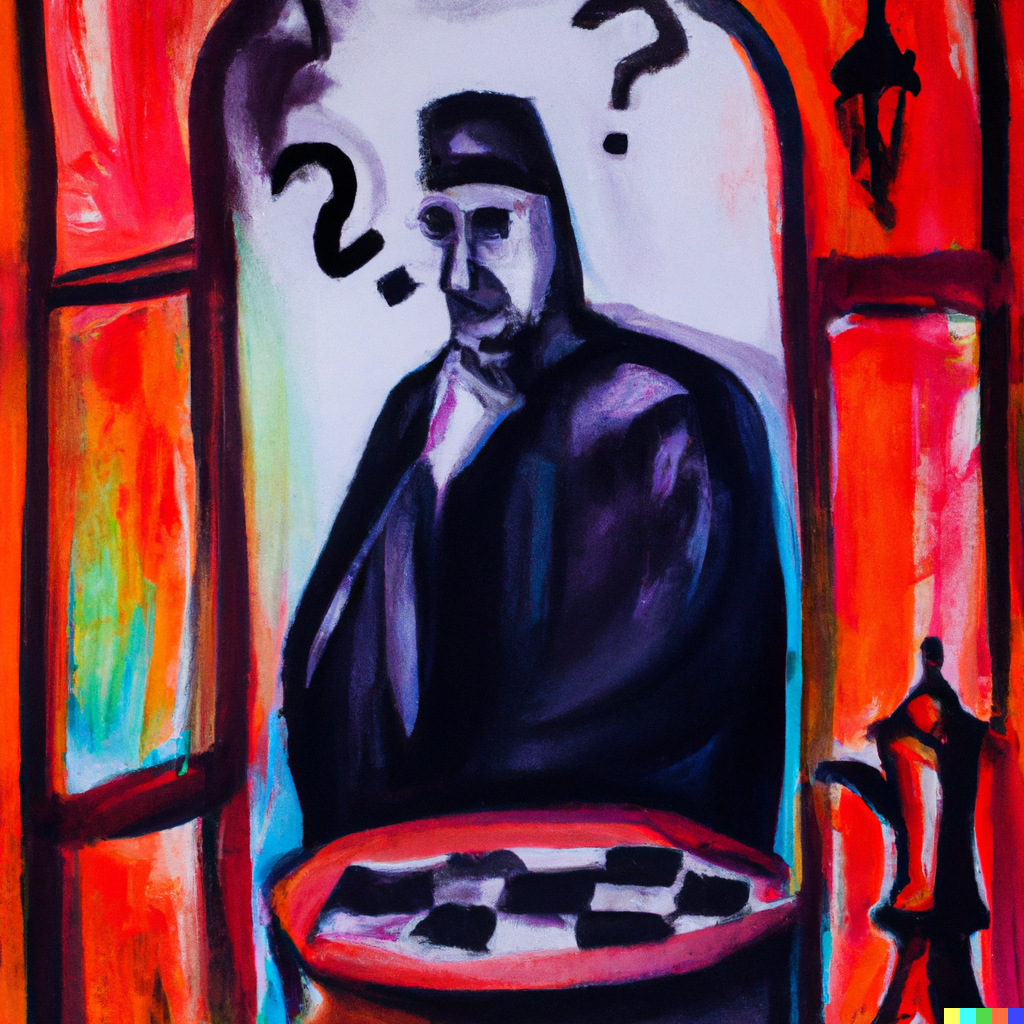
\includegraphics[width=0.5\textwidth]{Turingmachine/turing.png}
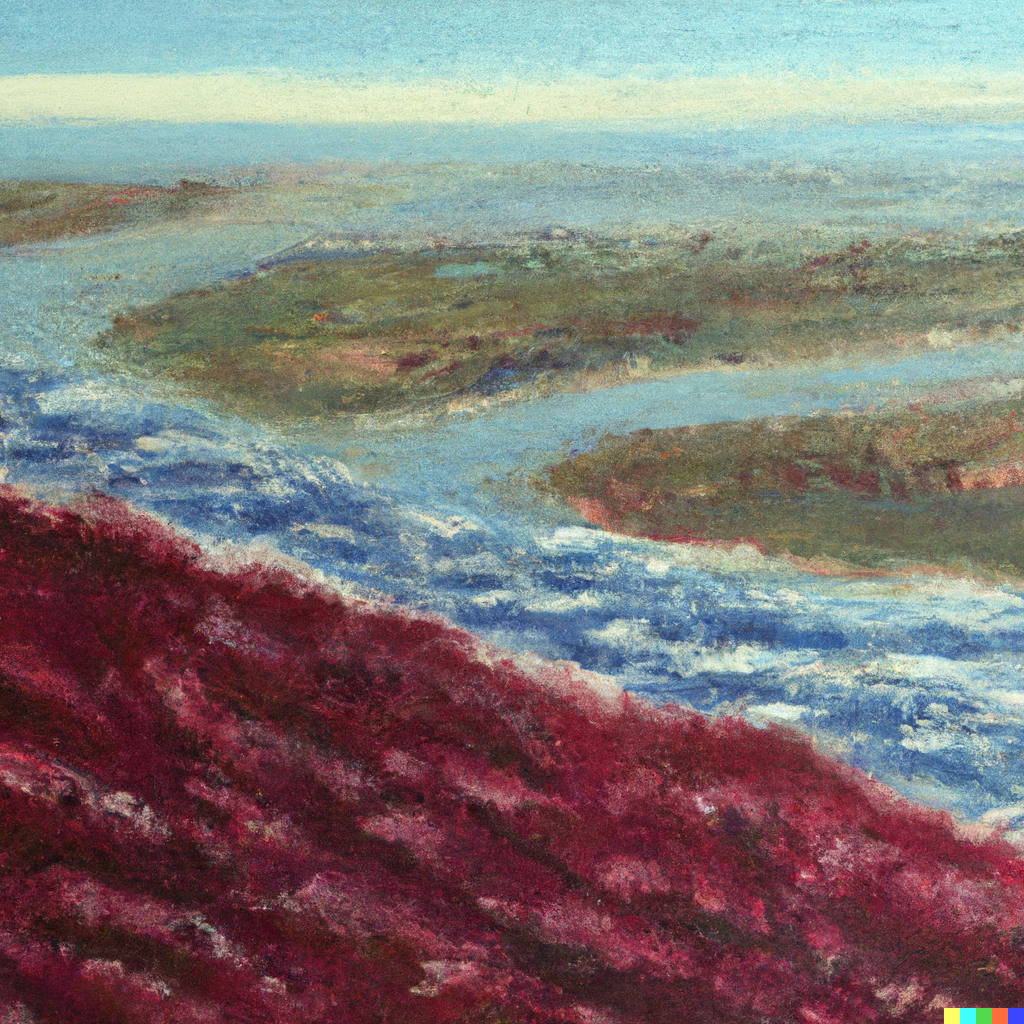
\includegraphics[width=0.5\textwidth]{Berechenbarkeit/predic.png}
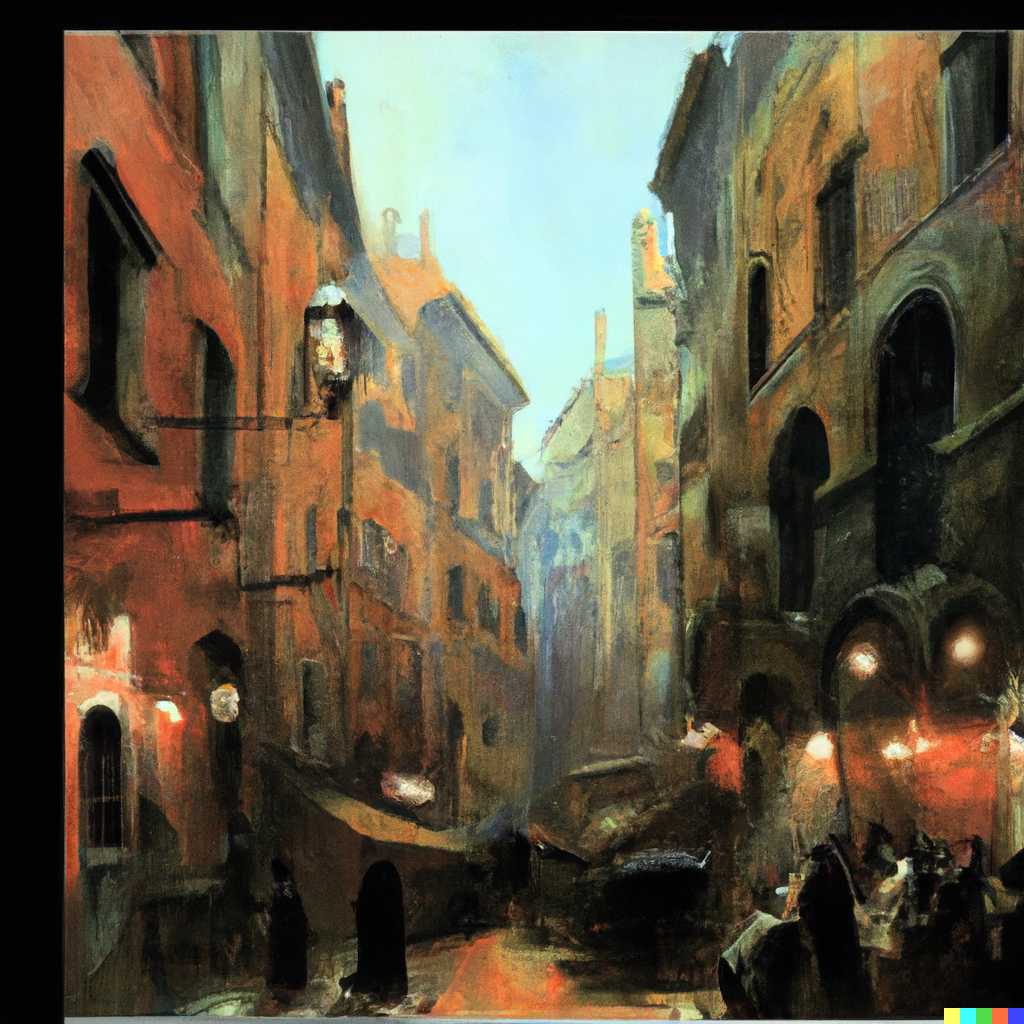
\includegraphics[width=0.5\textwidth]{Automaten/finit1.png}
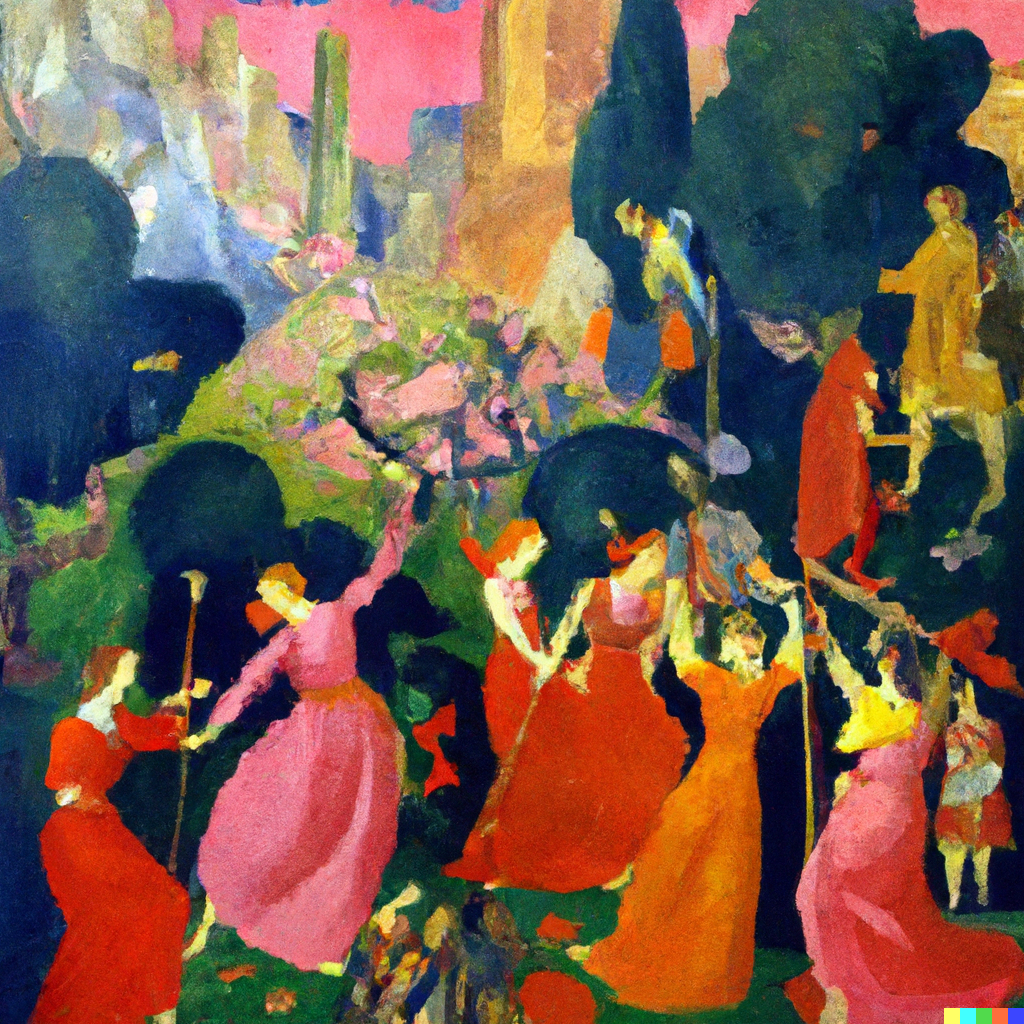
\includegraphics[width=0.5\textwidth]{ReguläreSprachen/regul.png}
%\includegraphics{}



\end{document}